\documentclass[12pt]{article}

% House style preamble
\input{.house-style/preamble.tex}
\usepackage{tikz}
\usetikzlibrary{arrows.meta,positioning}
\setlength{\emergencystretch}{3em}

% Toggle for blind review: set to true before submission
\newif\ifblind
\blindfalse  % \blindtrue for anonymous journal submission; \blindfalse for preprints

% Update PDF metadata
\ifblind
\hypersetup{
  pdftitle={What English Interjections Let Us Predict: Stable Causal-Pragmatic Clustering and Path Dependence},
  pdfauthor={}
}
\else
\hypersetup{
  pdftitle={What English Interjections Let Us Predict: Stable Causal-Pragmatic Clustering and Path Dependence},
  pdfauthor={Brett Reynolds}
}
\fi

\title{What English Interjections Let Us Predict:\\
Stable Causal-Pragmatic Clustering and Path Dependence}
\ifblind
\author{[Author removed for blind review]}
\else
\author{Brett Reynolds \orcidlink{0000-0003-0073-7195}%
\thanks{Contact: \href{mailto:brett.reynolds@humber.ca}{brett.reynolds@humber.ca}}\\
Humber Polytechnic \& University of Toronto}
\fi
\date{\today}

\begin{document}
\maketitle

\begin{abstract}
Is \term{interjection} a genuine lexical category of English? Grammars
have doubted it, and the doubt is about standing rather than about how
much has been written. This paper argues that the category earns its
place, and that what earns it isn't a defining property but
projectibility, which is the inferential payoff by which observing some
properties of a case licenses, namely warrants as a defeasible default,
predictions about others. Membership licenses inferences about
prosodic packaging, supplement function,
use-conditional stance, sequential position, response function, and
interactional uptake. Those inferences are pragmatic rather than
truth-conditional, which is a result about the category and not a change
of subject.

The paper argues that they're licensed by a stable causal-pragmatic
cluster. Invocative, verbal, and onomatopoeic routes recruit forms into a
similar profile, while leaving different pathway residues.
Regional/indexical conditioning supplies a further source of boundary
structure. Supplementary Corpus of Global Web-Based English (GloWbE) and
Corpus of Historical American English (COHA) probes illustrate boundary
behaviour, exit residue, and attrition. The result is a path-dependent
account of category membership: English interjections are projectible
because their prosodic, syntactic, semantic, and interactional
diagnostics are linked.
\end{abstract}

\noindent Keywords: interjections; lexical categories; category status;
projectibility; supplements; path dependence

% CONFIRM MODEL LIST: carried over verbatim from the end-of-paper
% declaration in the JoP submission, which named only "Claude (Anthropic)".
% The project's own session notes also record ChatGPT and Elicit at the
% review-board stage (STATUS.md, 2026-03-22). Decide whether those belong
% here and whether to name versions.
\aidisclosure{Claude (Anthropic)}

\section{Introduction}\label{sec:intro}

English interjections are small forms with large consequences. A
speaker's \mention{oh}, \mention{wow}, \mention{hey}, \mention{damn}, or
\mention{mm-hm} can package a response, display stance, open or sustain a
sequence, initiate repair, or invite uptake. Grammars have never been
settled about what to do with them. This paper asks whether
\term{interjection} is a genuine lexical category of English, and what
a form's membership in it licenses us to predict.

In 1586, William Bullokar wrote the earliest grammar of English. It
included interjections, which Bullokar defined as words that betoken
\enquote{a sudden passion of the mind} \citep[373]{bullokar1586}.

Four centuries later the standing is less secure.
\textcite[90]{jespersen1924} treated interjection as a manner in which
words of other categories may be used, which is to deny it categoryhood.
\textcite[67]{quirk1985} kept the category but called it
\enquote{marginal and anomalous}.
\textcite[22]{HuddlestonPullum2002} listed interjection as one of nine
lexical categories in \textit{The Cambridge Grammar of the English
Language} (\textit{CGEL}) (\mention{ah},
\mention{damn}, \mention{gosh}, \mention{hey}, \mention{oh},
\mention{ooh}, \mention{ouch}, \mention{whoa}, \mention{wow}), while the
companion textbook set it aside as \enquote{the minor category of
interjections \dots\ about which there really isn't anything interesting
for a grammar to say} \citep[16]{HuddlestonPullum2005}. Its second
edition returns interjection to the inventory, but concedes that
\enquote{grammarians typically say very little about interjections, and
we don't plan to be an exception} \citep[24]{HuddlestonPullumReynolds2022}.
Readmitted to the list, and still largely undescribed.

\textcite{libert2019} objects that calling interjections neglected
\enquote{is an overstatement}, and that's fair: work on their phonetics,
syntax, semantics, and pragmatics goes back a long way. What's stayed
unsettled is standing rather than volume of attention, namely whether
interjections constitute a category, and what membership would license.

The empirical picture hasn't simplified. English interjections span
phonology, morphology, syntax, semantics, and pragmatics. The
category resists clean definition, since no single property is necessary
and sufficient, and its boundaries with nouns, verbs, adverbs,
fillers, and routine formulae are graded rather than sharp.
Cross-linguistically, \enquote{interjection} is at best a comparative
concept \citep{haspelmath2010}.

Those difficulties are what make the category question worth asking. If
interjections are a category, the relevant payoff isn't an essence or a
single defining feature. It's \term{projectibility}: the inferential
payoff by which observing some properties of a new case licenses
predictions about others \citep{Goodman1955}. For interjections,
prosodic isolation, supplement function, or stance display should
license expectations about non-inflection, non-referential or
use-conditional meaning, sequential position, response function, and
interactional uptake.

Two terms need fixing before they start doing work. A form's
\term{profile} is the particular combination of cluster properties it shows
in a given grammatical environment: whether it's prosodically set off,
whether it inflects, whether it refers, what stance or response it carries.
The word is doing bookkeeping here and has nothing to do with the
figure-and-base sense familiar from cognitive grammar. And to say that a
property or a category \term{licenses} an inference is to say the inference
is a good default, defeasible by the particular case, not that it follows
necessarily.

The object of analysis is the category position, not the membership list
alone. Individual items such as \mention{wow}, \mention{damn},
\mention{bruh}, and \mention{fie} matter because they show what the
category licenses inference to: likely prosody, syntactic independence,
limits on argumenthood, stance or response function, and possible routes
into or out of the profile.

By \term{path dependence}, I mean that where a form came from keeps
showing in how it behaves at the category's edges, long after it has
arrived. \mention{Damn} came in from a verb and still takes a complement
(\mention{damn these mosquitoes!}); \mention{gee} came in by clipping a
religious invocation and takes nothing at all. Both sit squarely in the
profile, and they'd be indistinguishable if convergence erased history. It
doesn't, and that's useful in both directions: the leftovers of a form's
source let an analyst reason backwards from how a form behaves now to where
it came from.

Throughout, I use \term{property cluster} descriptively for the
empirical pattern of co-occurring features. English interjections form a
\term{stable projectible cluster} and a \term{causal-pragmatic kind}: a
category whose strongest inferences concern use, stance, sequence, and
uptake.

This inferential framing motivates a causal-network analysis.
\textcite{khalidi2013,khalidi2018nodes} argues that natural kinds are
nodes in causal structures rather than sets defined by essences. On
this account, a category is theoretically useful when its place in a
causal network supports reliable induction. Applied to interjections,
the claim is that several diagnostics, including prosodic isolation,
syntactic independence, non-referentiality, non-inflection, and
interactional force, cohere because several causal pathways converge on
the same pragmatic node. The resulting profile is thin but projectible.

The evidential order matters. The analysis first identifies a
\term{projection target}, namely what an analyst may infer from a form's
categorization as an interjection, and what speakers and hearers may
anticipate from partial cues without categorizing at all. Four further
questions follow, and because each has a label I'll use throughout, each is
worth stating plainly here.

\begin{itemize}
\item A \term{stable profile} is the same combination of properties
  recurring across forms and over time, rather than varying case by case.
\item \term{Network order} is a claim that those properties are linked to
  one another, so that the combination isn't a coincidence. A link here says
  that one property makes another more available, not merely that the two
  co-occur.
\item \term{Stabilizers} are processes that hold the combination together,
  so that it persists as individual forms enter and leave.
\item \term{Corrective control} is the strongest of these: a stabilizer
  that actively restores the combination when something disturbs it. Only
  this would license calling the cluster \term{homeostatic} (the term comes
  from Boyd's work on natural kinds, discussed in
  Section~\ref{sec:causal-framework}), and I don't claim it.
\end{itemize}

Diachrony matters because pragmatic profiles have histories. Forms such
as \mention{gee}, \mention{damn}, or \mention{bruh} change category
position as historically contentful or addressive expressions come to
manage stance, sequence, and interactional alignment in recurrent
contexts \citep[cf.][]{juckertaavitsainen2013}. Change over time helps
explain why the pragmatic profile is stable while individual forms enter,
leave, and retain source-specific residues.

The network classifies lexical items in grammatical environments, not
word families as wholes. A word family can contain distinct historically
related lexemes. The \mention{damn} word family includes verbal
\mention{damn} in \mention{I damn you} and standalone interjectional
\mention{damn!}. Prenominal \mention{damn} in \mention{the damn car}
belongs to that family too, but the analysis needn't decide here whether
it's a noun-phrase-internal extension of the interjection lexeme or a
separate adjectival lexeme. What matters is that it's syntactically
integrated inside a noun phrase while retaining use-conditional
expressive force.

The label \enquote{interjection} covers the overlap among
three partly overlapping nodes: a syntactic node, a semantic or
use-conditional node, and an interactional-pragmatic node. I write these
as \term{interjection\textsubscript{syn}},
\term{interjection\textsubscript{sem}}, and
\term{interjection\textsubscript{int}}. The sections below first
describe the diagnostic cluster, then explain why these nodes overlap
and why they come apart.

Section~\ref{sec:cluster} documents the cluster.
Section~\ref{sec:causal-framework} introduces the causal-network
framework that explains why the interjection profile supports pragmatic
inference. The rest of the paper identifies the network order that
structures the cluster, extends \textcite{gehweiler2008}'s single-case
analysis to a general claim about path dependence, and argues that
interjections exhibit a distinctive form of projectibility, primarily
pragmatic rather than truth-conditional.

\section{The property cluster}\label{sec:cluster}

English interjections exhibit a cluster of co-occurring properties across
phonology, morphology, syntax, semantics, and pragmatics. This section
surveys those properties, drawing primarily on the empirical base documented
in \textcite{ameka1992}, \textcite{quirk1985}, and
\textcite{HuddlestonPullum2002}. It answers two questions: what
properties cluster, and what local diagnostic inferences each property
supports. These inferences show that individual properties are
structured rather than accidental. Section~\ref{sec:projectibility} asks
the stronger question: when does a partial observation license inference
across linguistic domains? The causal question, why these properties
travel together, is deferred to Section~\ref{sec:causal-structure}.

\subsection{Phonology}

Interjections are prosodically isolated. They typically occupy their own
intonation unit, separated from surrounding discourse by pauses
\citep[108]{ameka1992}. In writing, this isolation surfaces as punctuation
(commas, dashes, exclamation marks), setting the interjection off from the
clause it accompanies \citep[1350]{HuddlestonPullum2002}.

The corpus evidence below is written, so prosodic isolation is tracked
through proxies: punctuation, standalone position, and absence of
integration into the host clause. These proxies are useful for historical
and large-corpus work, but they're proxies rather than direct acoustic
evidence.

Interjections may also contain phonemes outside the
speaker's dialect. The interjection \mention{uh-oh} ([\ipa{əʔo}]) is one of
the few cases where a glottal stop appears in dialects that otherwise lack
it. Other atypical sounds include the alveolar clicks in
\mention{tut-tut} ([\ipa{ǀǀ}]), the voiceless bilabial fricative in
\mention{whew} ([\ipa{ɸɪu}]), and (for dialects that no longer use it)
the voiceless velar fricative in \mention{ugh} ([\ipa{əx}])
\citep[853]{quirk1985}. Spelling pronunciations often arise for these forms
(e.g., [\ipa{tət tət}] for \mention{tut-tut}, [\ipa{əɡ}] for
\mention{ugh}), suggesting that the atypical phonemes are marked even for
native speakers.

Prosodic isolation is a strong cue: if
a novel form occupies its own intonation unit and resists integration into
the surrounding prosodic contour, a listener can predict syntactic
non-integration and non-referentiality. The atypical phonemes reinforce this
inference. But prosodic isolation isn't unique to interjections, since
vocatives, appositives, and other supplements share it \citep[cf.][]{wilkins1992}. What
distinguishes interjections is the convergence of prosodic isolation with
the properties below.

\subsection{Morphology}

English interjections characteristically don't inflect or derive. They
resist the morphological operations that characterize other open-class
categories: no plural (*\mention{ouches}), no tense (*\mention{ouched}),
no comparative (*\mention{oucher}), no nominalization
(*\mention{ouchness}) \citep[106]{ameka1992}. Since
\textcite{libert2019} notes that \enquote{few, if any, papers focus on
the morphology of interjections}, the apparent absence of morphological
productivity may partly reflect a gap in the research rather than a
firm empirical generalization.

Some interjections retain remnants of earlier categorial membership.
\mention{Heavens} and \mention{bollocks} preserve the nominal plural
suffix. \mention{Goddammit} preserves a verb-object-pronoun structure,
which is fossilized syntax rather than morphology, and belongs with the
syntactic residue discussed in Section~\ref{sec:cluster}. None of these
remnants are productive. The plural in
\mention{heavens} doesn't contrast with a singular *\mention{heaven!} (as
an interjection), and speakers don't extend the pattern to new forms.

Non-inflection predicts
non-argumenthood. Forms that don't inflect can't control verb agreement or take
a determiner, so they can't fill the syntactic slots that require these
operations. But non-inflection alone isn't diagnostic: adverbs also don't
inflect \citep[106]{ameka1992}. The stronger diagnostic is syntactic:
adverbs characteristically form constituents with other words, while
canonical interjections occur as standalone supplements and resist
integration with neighbouring material \citep[152]{meinard2015}.

\subsection{Syntax}

Interjections characteristically function as \term{supplements},
\enquote{elements which occupy a position in linear sequence without
being integrated into the syntactic structure of the sentence}
\citep[1350]{HuddlestonPullum2002}. In \mention{Damn, we're going to be late!}, the
interjection isn't a complement or modifier of anything in the clause.
It's appended to the beginning as a parenthetical.

Supplement function isn't unique to interjections. Relative clauses, noun
phrases, adjective phrases, and adverb phrases can all function as
supplements \citep[1356--1360]{HuddlestonPullum2002}:

\ea\label{ex:supplements}
  \ea \mention{Ah}, so you were there after all! \hfill (interjection, p.~1360)
  \ex We called in to see Sue's parents, \mention{which made us rather late}. \hfill (relative clause, p.~1356)
  \ex A university lecturer, \mention{Dr Brown}, was arrested for the crime. \hfill (noun phrase, p.~1357)
  \z
\z
What distinguishes interjection supplements is their combination with
the other cluster properties: non-referentiality, non-inflection,
prosodic isolation, and emotive force. The function is shared; the
category differs.

A handful of interjections exceptionally take complements.
\textcite[1361fn]{HuddlestonPullum2002} analyse \mention{damn} in
\mention{damn these mosquitoes!} as the head of an interjection phrase
(IntjP) taking a noun phrase (NP) complement, one of the very few cases where an
interjection projects beyond a single word. But even here the syntax is
constrained: no subject is present or intended, and there's no tense
inflection. The construction is better treated as a residue of verb
syntax than as full verbal behaviour, a point that matters for the
recruitment pathways
discussed in Section~\ref{sec:causal-structure}. (The internal structure of
lexicalized pairs like
\mention{oh boy} and \mention{holy cow} is less clear and won't be
resolved here.)

Supplement function predicts prosodic isolation and resistance to
syntactic integration:

\ea\label{ex:syntactic-predictions}
  \ea[*]{\mention{I think that damn we're going to be late.}}
  \ex \mention{I think that, damn, we're going to be late.}
  \ex[*]{\mention{Damn and quickly, we left.}}
  \z
\z
Supplement function also predicts a semantic consequence: if the form is
syntactically non-integrated, its contribution is independent of the
proposition expressed by the host clause. Remove the interjection and the
truth conditions don't change, the hallmark of non-truth-conditional
meaning \citep[cf.][166]{potts2007}.

\subsection{Semantics}

English interjections characteristically don't refer. Here,
\term{non-referentiality} means absence of ordinary entity/event
denotation and argumental construal while allowing semantic content.
Nouns and verbs typically pick out entities or events in the world.
Interjections express internal states of their users
\citep{leech2006}: anger (\mention{damn}),
disgust (\mention{eww}, \mention{yuck}), surprise (\mention{wow}), regret
(\mention{alas}), pain (\mention{ouch}), realization (\mention{eureka}).
Some interjections are more propositional than emotive: \mention{yes}
and \mention{no} affirm or deny propositions, and \mention{oh} can
signal recognition of new information rather than expressing feeling.

\textcite{wierzbicka1992} argues that interjections have genuine
semantic content, decomposable via Natural Semantic Metalanguage into
deictic primitives (\mention{I}, \mention{you}, \mention{now},
\mention{here}). That remains compatible with the definition above. The
forms may have content, and \mention{yes} and \mention{no} may operate
on propositions, while still lacking ordinary entity/event denotation.
Wierzbicka's explications characterize the use-conditional content that
\term{interjection\textsubscript{sem}} (Section~\ref{sec:fieldrelative-nodes})
tracks. Non-referentiality is a cluster property rather than a
definition.

The contrast with nouns is sharpest where both share a lexical source.
\mention{Jesus} as a noun refers to a person; \mention{Jesus!} as an
interjection doesn't. In the interjection use, as
\textcite[88]{gehweiler2008} puts it, \mention{Jesus} \enquote{has lost
its propositional content, i.e.\ it is no longer used to refer and hence
no longer influences truth conditions}.
This semantic shift is part of the recruitment pathway from noun to
interjection (Section~\ref{sec:causal-structure}).

The projectibility here is mostly negative. A form that doesn't refer
resists being made definite, quantified over, or used as an argument:
*\mention{the damn!}, *\mention{every ouch}, *\mention{Damn surprised me},
and *\mention{There's damn}. These restrictions are non-trivial because
they distinguish interjections from nouns that have undergone only partial
bleaching. Section~\ref{sec:synchronic-coupling} treats the same relation from
the causal side: non-referentiality helps keep the form out of
argument structure, which in turn supports prosodic isolation.

\subsection{Pragmatics}

Interjections typically carry exclamatory or imperative force: \mention{ouch!}
expresses pain, \mention{shh!} demands silence \citep[88]{quirk1985}. But
the pragmatic range extends beyond exclamation. Interjections greet
(\mention{hey}, and, at the boundary with routine formulae,
\mention{hello}; see Section~\ref{sec:boundaries}), mark agreement (\mention{yes},
\mention{amen}), indicate understanding (\mention{oh}, \mention{uh-huh}),
and signal backchanneling, the listener's ongoing attention to a speaker's
turn \citep{dingemanse2020, stivers2019}.

The most common interjections tagged in the Corpus of Global Web-Based
English \citep[GloWbE;][]{daviesfuchs2015} illustrate this pragmatic breadth: \mention{yes}, \mention{no},
\mention{oh}, \mention{yeah}, \mention{hi}, \mention{hey}, \mention{wow},
\mention{hello}, \mention{ah}, \mention{ha}. The list is dominated by
interactional items, forms whose primary function is to manage the
conversation rather than to contribute propositional content.
\textcite{dingemanse2024} estimates that roughly one in seven
conversational turns is an interjection, and interactional tools
dominate the most frequent cases: continuers like
\mention{mm-hm} that scaffold extended turns, repair initiators like
\mention{huh?} that calibrate mutual understanding, and change-of-state
tokens like \mention{oh} that display evolving knowledge\footnote{%
  \term{Token} does double duty in work of this kind, and I keep the senses
  apart. In \term{change-of-state token} and \term{response token} it's the
  interactional-linguistic sense: a minimal form deployed as a move in a
  sequence. Elsewhere I use it for the unit of analysis, a lexical item in a
  grammatical environment as against the lexeme that labels a family of
  historically related such items.}
\citep[cf.][]{norrick2009}.

The boundary with \term{routine formulae} is instructive.
\textcite[2--3]{coulmas1981} defines routine formulae as
% "conventionalised" is Coulmas's British spelling, preserved as quoted;
% verified via Ameka's verbatim reproduction at p. 108, same page range.
\enquote{highly conventionalised prepatterned expressions whose occurrence
is tied to more or less standard communication situations}:
\mention{bye}, \mention{hello}, \mention{sorry}, \mention{thank you}.
\textcite[109--110]{ameka1992} argues these differ from interjections in
three ways: they include addressees, they're predictable responses to social
conventions, and they're always speech acts rather than mere reflections of
the speaker's mental state. \textcite[142]{wilkins1992} counters that these
differences make routine formulae \enquote{a distinct pragmatic and semantic
subtype of interjections}, not a separate category.

The disagreement is field-relative in a causal-network sense. For a
grammar, routine formulae pattern near interjections because they share
prosodic isolation and pragmatic function. For speech-act analysis or
interactional pragmatics, they support different predictions: addressee
orientation, occurrence in standard social sequences, and conventional
felicity conditions. The same form can sit close to one node
for one inquiry and farther away for another, depending on which causal
relations and predictions the inquiry tracks.

The projective claim should be level-specific. A novel
non-propositional stance form licenses expectations about standalone
positioning, supplement-like syntax, backchannel availability, and
resistance to embedding under reported speech (\mention{*She said that
damn}). A novel routine formula licenses expectations about
addressee-directedness and placement in conventional social sequences.
The overlap explains why routine formulae sit at the boundary; the
divergence explains why the boundary is disputed.
Section~\ref{sec:causal-structure} asks which links make those claims
reliable.

\subsection{Co-occurrence, not necessity}\label{sec:cooccurrence}

These properties co-occur statistically, not necessarily. The
literature's own definitions hedge, and the hedges are the point.
% Verified verbatim against Wilkins 1992: 124 (running head "124 D. P.
% Wilkins / Interjections as deictics"), his numbered definition (1).
% Note: Gehweiler's block quote at p. 73 pluralizes "construction"; the
% singular here follows Wilkins directly.
\textcite[124]{wilkins1992} defines an interjection as
\enquote{a conventional lexical form which (commonly and) conventionally
constitutes an utterance on its own, (typically) does not enter into
construction with other word classes, is (usually) monomorphemic, and
(generally) does not host inflectional or derivational morphemes}. Four
criteria, a parenthetical hedge on each, and
\textcite[73]{gehweiler2008} adopts the definition while calling those
criteria the class's \enquote{obligatory properties}. No single property
is necessary and sufficient.

The pattern calls for explanation. Network order couples the
properties: prosodic isolation reinforces syntactic non-integration,
non-referentiality removes the need for argument structure, and
pragmatic conventionalization entrenches the emotive function.

The coupling is visible when it breaks. \mention{Damn} as an interjection
(\mention{Damn!}) has the full cluster: prosodic isolation, syntactic
non-integration, non-referentiality, and emotive force. Prenominal
\mention{damn} in \mention{the damn car} retains emotive force but
loses prosodic-syntactic independence because it's embedded inside an
noun phrase \citep[cf.][]{potts2007}. When that link is neutralized, the
properties erode together. A bare property list can't explain this
pattern; a process-linked cluster explains it.

Table~\ref{tab:diagnostic-matrix} makes the cluster inspectable.
Each row gives a lexical item in a grammatical environment rather than
a word family as a whole (see Section~\ref{sec:intro}), and the columns show its
profile against the five cluster properties and the three field-relative
nodes previewed in the introduction and defined in
Section~\ref{sec:fieldrelative-nodes}. The compact labels
Intj\textsubscript{syn}, Intj\textsubscript{sem}, and
Intj\textsubscript{int} refer to syntactic, semantic/use-conditional,
and interactional-pragmatic interjection nodes, respectively. The table
shows convergence and decoupling. Standalone \mention{damn!} and
\mention{oh} show convergence. In \mention{the damn car}, prenominal
\mention{damn} has the semantic node but lacks the syntactic one.
\mention{mm-hm} has the interactional node, while its syntactic status
is debatable. Boundary items (\mention{bye}, \mention{um}) share some
but not all cluster properties, the pattern that
Section~\ref{sec:boundaries} explains as causal-link overlap.

\begin{table}[htbp]
\centering
\footnotesize
\caption{Diagnostic matrix: constructions against cluster properties and
field-relative nodes. \checkmark\ = property present; ($\checkmark$) =
partial or debated; \textendash{} = absent. Intj\textsubscript{syn},
Intj\textsubscript{sem}, and Intj\textsubscript{int} abbreviate
syntactic, semantic/use-conditional, and interactional-pragmatic nodes.
Sources:
properties from
\textcite{ameka1992}, \textcite{quirk1985},
\textcite{HuddlestonPullum2002}; \term{interjection\textsubscript{sem}} from
\textcite{potts2007}; \term{interjection\textsubscript{int}} from
\textcite{stivers2019}, \textcite{dingemanse2020}.}
\label{tab:diagnostic-matrix}
\begin{tabular}{@{}l*{5}{c}c*{3}{c}@{}}
\toprule
 & \rotatebox{70}{Prosodic isol.}
 & \rotatebox{70}{Non-inflecting}
 & \rotatebox{70}{Synt.\ non-int.}
 & \rotatebox{70}{Non-referential}
 & \rotatebox{70}{Emotive/stance}
 & \phantom{x}
 & \rotatebox{70}{Intj\textsubscript{syn}}
 & \rotatebox{70}{Intj\textsubscript{sem}}
 & \rotatebox{70}{Intj\textsubscript{int}} \\
\midrule
\mention{gee!}
  & \checkmark & \checkmark & \checkmark & \checkmark & \checkmark
  && \checkmark & \checkmark & \checkmark \\
\mention{damn!}
  & \checkmark & \checkmark & \checkmark & \checkmark & \checkmark
  && \checkmark & \checkmark & \checkmark \\
\mention{damn these \ldots!}
  & \checkmark & ($\checkmark$) & ($\checkmark$) & \checkmark & \checkmark
  && ($\checkmark$) & \checkmark & \textendash{} \\
\mention{the damn car}
  & \textendash{} & \textendash{} & \textendash{} & \textendash{} & \checkmark
  && \textendash{} & \checkmark & \textendash{} \\
\mention{oh}
  & \checkmark & \checkmark & \checkmark & \checkmark & \checkmark
  && \checkmark & \checkmark & \checkmark \\
\mention{mm-hm}
  & \checkmark & \checkmark & \checkmark & \checkmark & ($\checkmark$)
  && ($\checkmark$) & \textendash{} & \checkmark \\
\mention{huh?}
  & \checkmark & \checkmark & \checkmark & \checkmark & ($\checkmark$)
  && ($\checkmark$) & \textendash{} & \checkmark \\
\mention{bruh}
  & \checkmark & \checkmark & \checkmark & \checkmark & \checkmark
  && \checkmark & \checkmark & \checkmark \\
\mention{bye}
  & \checkmark & \checkmark & \checkmark & ($\checkmark$) & \textendash{}
  && \checkmark & \textendash{} & ($\checkmark$) \\
\mention{um}
  & ($\checkmark$) & \checkmark & \checkmark & \checkmark & \textendash{}
  && ($\checkmark$) & \textendash{} & ($\checkmark$) \\
\bottomrule
\end{tabular}
\end{table}

The next two sections develop the theoretical framework
(Section~\ref{sec:causal-framework}) and the causal structure itself
(Section~\ref{sec:causal-structure}).

\section[Pragmatic projectibility]{Explaining pragmatic projectibility}\label{sec:causal-framework}

The property cluster documented above has a distinctive shape:
statistically reliable co-occurrence, no necessary and sufficient
conditions, graded boundaries, and hedged universals. That profile is
exactly what makes interjections valuable for pragmatics. The label
\enquote{interjection} supports predictions about use, but those
predictions cross phonology, syntax, semantics, interaction, and
diachrony. Causal-network analysis explains why those inferences are
available without treating the category as an essence.

\subsection{The framework}

\textcite{khalidi2013,khalidi2018nodes} argues that natural kinds are
nodes in causal structures. A kind can be unified by causal relations
rather than by an essence. Those relations may be local
mutual-reinforcement relations, one-directional pathways, or converging
historical routes. What matters is that the category marks a place in a
causal network: a position where properties, processes, and
interventions are connected tightly enough to support induction. The
clustering matters because it lets us predict properties of new
instances from observed properties of old ones.

The claim is methodological rather than metaphysically heavyweight.
Interjections need not be \enquote{genuine kinds} in the strongest
sense. The category only needs to be a projectible kind for linguistic
inquiry: a node whose causal links explain why particular observations
support particular predictions.

I use the framework as a diagnostic ladder\ifblind\else\
\citep{reynolds2026notEveryStableCluster}\fi. First, what's the
\term{projection target}: the field-relative inference the category is
supposed to support? Second, what \term{stable profile} supports that
target? Third, what \term{network order} makes the profile
non-accidental? Fourth, what \term{stabilizers}, if any, keep the
profile available across relevant contexts? Fifth, is any stabilizer a
\term{controller}: a perturbation-sensitive process that corrects
departures from the profile? Projectibility is the payoff; strict
homeostasis is the final and most demanding evidential claim.

The framework also clarifies how the argument relates to
\term{homeostatic-property-cluster theory}. \textcite{boyd1999} showed
that fuzzy categories can be useful and projectible when their
properties are connected non-accidentally. Interjections have that shape:
they lack necessary and sufficient conditions, but show recurrent
co-occurrence among prosodic, syntactic, semantic, and pragmatic
diagnostics. The question is how strong a causal claim that recurrence
supports.

Some relevant properties form local stabilizing relations. Prosodic
isolation and syntactic non-integration reinforce one another: a form
produced as its own intonation unit is less available for complementation
or modification, while a form outside clause structure is more likely to
receive independent prosodic packaging. Repeated use in that position can
make standalone interpretation increasingly expectable for speakers and
hearers.

Other processes are interactional or directional. Uptake affects future
use; repeated use affects expectation; expectation affects later uptake.
Loss of referential content makes argument structure less motivated;
syntactic deactivation pushes a form toward standalone use; repeated
conversational deployment entrenches stance, response, repair, or
sequence-management functions. These relations explain why the
diagnostics travel together. They establish network order and plausible
maintenance rather than homeostasis
\citep[cf.][]{weinberger2026HomeostasisCausalControl}.

The historical evidence adds a further point. Semantic bleaching,
syntactic deactivation, and onomatopoeic or interactional coinage can all
recruit forms into a similar pragmatic profile, but they don't do so by
the same route or with the same residues. A bleached invocation, a
deactivated imperative, and an onomatopoeic or interactional form may
converge on prosodic independence, supplement function,
non-referential or use-conditional meaning, and interactional force while
retaining different traces of their sources. The resulting category is
organized by causal-pragmatic relations with different temporal and
explanatory profiles.

That structure is enough for pragmatic projectibility, but not enough
for strict homeostasis. The evidence considered here doesn't identify a
tracked category-level variable, an error signal, or a response pathway
that restores the interjectional profile when it's perturbed.
Interjections are stable and projectible because their diagnostics are
linked within a causal-pragmatic structure.

\subsection{Causal networks vs.\ prototype theory}

Prototype theory \citep{rosch1975,taylor2003} was developed for exactly
the kind of data Section~\ref{sec:cluster} documents, and it handles
that data well: graded membership, better-and-worse exemplars, and
fuzzy boundaries via overlapping similarity spaces. It also correctly
predicts that boundary disputes (interjections vs.\ fillers, vs.\
routine formulae) should recur instead of being resolvable by
definition. These are genuine explanatory achievements, and the
causal-network account doesn't replace them.

A causal-network account adds a different kind of question. Prototype
theory explains why borderline cases should be expected: categories are
organized around better and worse exemplars. It doesn't explain why
the properties cluster in this particular pattern or what should happen
when one of their links is disrupted.

The difference matters because the causal-network account generates
predictions about change, conditioning, and residues. It predicts that
forms recruited by different pathways should retain different traces of
their source constructions, that apparent gradience should decompose
under variety conditioning, and that some properties may be more central
to network order than others (hub-property asymmetry). These
predictions are probed for interjections in Section~\ref{sec:discussion}.

Pathway residues provide a further discriminator. If the proposed causal
links are real, messy boundary cases shouldn't be messy in arbitrary
ways. Retained complements should point to verbal sources; euphemistic
phonological deformation should point to taboo-managed invocative
sources; regional concentration should point to regional or indexical
recruitment. Prototype theory offers no analogous retrodictive test.

\subsection{What causal structure adds}

Several analytical stances generate different predictions for
interjections. The weakest is a \term{property list}: interjections share
prosodic isolation, non-inflection, non-referentiality, and emotive
force. That's descriptively useful, but it makes no prediction about
what happens when one property changes.

Feature specifications are stronger alternatives, for example
[\textsc{+peripheral}, \textsc{-argument-taking},
\textsc{+expressive}]. This generates some of the same distributional
consequences: no inflection follows from the absence of phi-features,
and no argument-taking follows from the relevant syntactic feature
bundle. But feature specifications treat those consequences as
entailments of the feature bundle, not as effects of identifiable
processes.

A constructional account is a stronger competitor. It can represent
many of the same pairings of form, meaning, and use
\citep{goldberg1995constructions,goldberg2006,croft2001}. The
causal-network claim is compatible with that representational move. It
asks a different question: which positions in a constructional inventory
are projectible, why do their properties cohere, and which changes
should make them come apart? Construction grammar models the inventory;
the causal-kind question asks where the inventory supports
cross-constructional and cross-field inference. The two main pressure
points are pathway residues and field-relative decomposition. If those
payoffs fail under further testing, the causal-network account collapses
to a descriptive inventory rather than an explanatory category analysis.

The causal-network account adds five claims that property lists, feature
bundles, and constructional representations don't settle by themselves:

\begin{enumerate}
\item Co-movement. Prosodic isolation, supplement function,
  non-referentiality, and pragmatic force recur in a patterned way. The
  account asks which links explain why observing one property licenses
  expectations about another.
\item Asymmetry. Some properties are upstream or more diagnostic than
  others. Prosodic packaging can make syntactic integration less
  available, while the reverse relation has a different status. A flat
  feature bundle can't represent that ordering.
\item Persistence. The category profile can remain available while
  individual forms enter and leave. That makes a stability claim while
  leaving homeostasis open.
\item Boundary behaviour. Different recruitment pathways should leave
  different residues at the category boundary. Feature theory can list
  residual properties but doesn't explain why they align with
  particular histories.
\item Failure. When a prediction fails, the pattern of failure should
  identify which link or projection target has broken. If \mention{fie}
  loses all three nodes together under community-wide attrition, the
  result is a boundary condition on ordered erosion rather than evidence of corrective
  control.
\end{enumerate}

If a feature-based account can replicate co-movement, asymmetry,
persistence, boundary behaviour, and failure without network order,
causal structure is doing no additional explanatory work. The empirical
pressure point is whether the probes in Section~\ref{sec:discussion}
support those claims.

\subsection{Field-relative projectibility}\label{sec:fieldrelative-nodes}

The causal-network account developed by
\textcite{khalidi2013,khalidi2018nodes} also explains why
projectibility is field-relative. If kinds are nodes in causal
structures, different fields may track different nodes because they ask
different explanatory and predictive questions. The resulting categories
remain realist: each inquiry tracks the causal relations that matter for
its explanations and predictions.

A parallel formulation in homeostatic-kind theory makes the point
explicit: \enquote{A kind may be natural \enquote{from the point of view
of} some discipline or disciplinary matrix, but not \enquote{from the
point of view of} another} \citep[160]{boyd1999}. I take that
formulation as a useful gloss on the causal-network account.

The familiar linguistic parallel is the interrogative/question
distinction. Syntacticians track \term{interrogative}: a clause type
with properties such as subject--auxiliary inversion, fronting of
interrogative words, and polar-question syntax. Pragmatists track \term{question}:
a speech act that requests information, projects an answer, and
organizes uptake. The two often coincide, and they also come apart:
\mention{Can you pass the salt?} is syntactically interrogative and
pragmatically a request, while \mention{I wonder where she went} can
raise an information issue without having interrogative clause syntax.

Interjections create a similar problem with less terminological help.
Syntax, semantics, and interactional pragmatics all use the
word \enquote{interjection}, but each field tracks a slightly different
node: different properties, different causal links, different
predictions. I distinguish these with subscripts:%
\footnote{The interrogative/question contrast uses different words for
  the syntactic and pragmatic nodes because both terms are established
  in their respective traditions. For interjections,
  every field uses the same word, so subscripts are the honest notation.
  An alternative would have been to adopt distinct terms from the
  relevant literatures: \term{expressive} from \textcite{potts2007}
  for the semantic node, and \term{response token} from
  \textcite{stivers2019} or \term{liminal sign} from
  \textcite{dingemanse2020} for the interactional-pragmatic node.

  The Latin
  \term{ejaculatio}, a throwing out, mirroring \term{interjicere},
  \enquote{to throw between} \citep{libert2019},
  would have been etymologically perfect
  for the interactional-pragmatic category, but modern English has
  rendered the term unavailable.}

\begin{itemize}
\item \term{interjection\textsubscript{syn}}, the syntactician's
  category (\textit{CGEL}, Quirk et al.). Distributional cluster: supplement
  function, non-inflecting, non-argument-taking. Linked by
  prosodic-syntactic coupling. Projects syntactic behaviour.
\item \term{interjection\textsubscript{sem}}, the semanticist's
  category, overlapping with \textcite{potts2007}'s \term{expressives}.
  Use-conditional meaning cluster: independent of at-issue content,
  nondisplaceable, perspective-dependent, descriptively ineffable
  \citep[166]{potts2007}. Often recruited through semantic bleaching.
  Projects meaning type. Different extension: prenominal \mention{damn} in
  \mention{the damn car} is \term{interjection\textsubscript{sem}} but not
  \term{interjection\textsubscript{syn}}.
\item \term{interjection\textsubscript{int}}, the interactional-pragmatic
  category, overlapping with \textcite{stivers2019}'s
  response tokens and \textcite{dingemanse2020}'s liminal signs.
  Sequential/stance cluster: turn-initial, backchannel, stance display.
  Linked by routine entrenchment and possibly by regional/indexical
  conditioning. Projects pragmatic behaviour in interaction. Different
  extension: \mention{mm-hm} is
  \term{interjection\textsubscript{int}} but debatably
  \term{interjection\textsubscript{syn}}.
\end{itemize}

The subscript notation makes explicit that these are overlapping but
non-identical nodes, each linked by different ordering or stabilizing
relations, and projectible for different purposes. The traditional label
\enquote{interjection} names their zone of overlap, and the paper's
remaining sections analyze that overlap from multiple angles.

\section[Causal structure]{Causal structure: recruitment and coupling}\label{sec:causal-structure}

The property cluster documented in Section~\ref{sec:cluster} raises two
questions that co-occurrence alone can't answer: how do items enter the
interjectional region of the network, and which causal links make the
properties travel together? In what follows, \enquote{the
interjection cluster} refers to the broad property profile. I use
\enquote{the intersection} only for cases that belong simultaneously to
\term{interjection\textsubscript{syn}}, \term{interjection\textsubscript{sem}}, and
\term{interjection\textsubscript{int}}.
A causal-network account requires both a diachronic account of
recruitment and a synchronic account of the network order among
properties.

Table~\ref{tab:link-status} sets out each proposed link with its current
evidential status, the kind of evidence that would bear on it, and the
main way it could fail.

\begin{table}[t]
\centering
\scriptsize
\caption{Status of the proposed ordering and stabilizing links}
\label{tab:link-status}
\begin{tabular}{@{}
  >{\raggedright\arraybackslash}p{.22\textwidth}
  >{\raggedright\arraybackslash}p{.20\textwidth}
  >{\raggedright\arraybackslash}p{.27\textwidth}
  >{\raggedright\arraybackslash}p{.23\textwidth}
  @{}}
\toprule
Link & Status & Evidence type & Main vulnerability \\
\midrule
Semantic bleaching from invocatives &
Historically documented &
Gehweiler-style corpus trajectory &
Operationalizing invocation versus exclamation. \\
\addlinespace
Syntactic deactivation from verbs and imperatives &
Plausible and reconstructive &
Residual complement structure, imperative frames, discourse-marker uses &
Needs fuller diachronic series. \\
\addlinespace
Onomatopoeic or liminal coinage &
Plausible entry route &
Synchronic profile of coined forms &
Coinage isn't the same kind of process as bleaching. \\
\addlinespace
Prosodic-syntactic coupling &
Stabilizer candidate, partly proxy-based &
Supplement syntax, punctuation, standalone position &
Written corpora underrepresent prosody. \\
\addlinespace
Non-referentiality ratchet &
Ordering link &
Argument-structure restrictions &
\mention{Yes}, \mention{no}, and response tokens complicate the property. \\
\addlinespace
Routine entrenchment &
Stabilizer candidate for \term{interjection\textsubscript{int}} &
Conversation-analytic and pragmatic literature &
Needs more spoken-interaction data for the present cases. \\
\addlinespace
Regional/indexical conditioning &
Maintenance hypothesis &
Regional concentration and register sensitivity &
Identity-work evidence remains outside the present data. \\
\bottomrule
\end{tabular}
\end{table}

\subsection{Recruitment pathways}\label{sec:recruitment}

Section~\ref{sec:cluster} already pointed to three recruitment
pathways: semantic bleaching from nouns, syntactic deactivation from
verbs, and nonce coinage via onomatopoeia. The first is historically
demonstrated; the second and third are proposed pathways with clear
examples but without the extended diachronic documentation that Path~1
has. The first two are analysed in detail here; the third is taken up
in Section~\ref{sec:turnover}.

The pragmatic issue is how changes in communicative use become
categorially consequential: grammaticalization and pragmaticalization
matter here because they alter a form's communicative job as well as its
position in a syntactic tree
\citep[cf.][]{TraugottDasher2002, heinekuteva2002lexicon}.

\subsection{Path 1: religious noun to interjection}

\textcite{gehweiler2008} traces the development of \mention{gee} from
\mention{Jesus} through three positions:

\ea\label{ex:bleaching}
  \ea Proper name used as invocation (\mention{Jesus!} addressed to the
    deity)
  \ex Secondary interjection: exclamatory use, no longer addressing the
    deity (\mention{Jesus!} as an expression of surprise)
  \ex Primary interjection: phonological modification yields
    \mention{Jeez} and \mention{Gee}, and \mention{gee!} detaches from
    the source noun
  \z
\z
The two transitions don't work the same way, and Gehweiler is emphatic
about the difference. She explains the first as gradual and speaker-based,
through Traugott and Dasher's invited inferencing, and
\enquote{advanced by the syntactic isolation of \mention{Jesus}}
\citep[85]{gehweiler2008}. The second she treats as abrupt and
hearer-based: tabooistic clipping produced \mention{gee!}, and she insists
that this step \enquote{was not gradual} and \enquote{can therefore not be
explained with reference to Invited Inferencing or syntactic position}
\citep[88]{gehweiler2008}.
The positions layer cluster properties unevenly. Prosodic isolation is
already present at the invocation, because a vocative like
\mention{Jesus!} occupies its own intonation unit (contrast the
integrated argument in \mention{Put your faith in Jesus}). What changes
is the content: non-referentiality arrives with the secondary interjection, when the speaker
is no longer addressing the deity. Phonological divergence then
makes the etymological connection opaque, and the result is a
standalone interjection that many speakers don't connect to its source.
For the first transition the vocative is the gateway: it provides the
prosodic isolation that bleaching exploits, so the prosodic slot was there
first and the semantic content drained out of it
\citep[85]{gehweiler2008}. Gehweiler denies that the same explanation
extends to the second.

That discontinuity is an asset for the path-dependence claim rather than
an embarrassment for it. A gradual slide would leave a form with no
particular mark of where it came from; an abrupt re-analysis leaves exactly
the kind of residue the account needs, since the phonological opacity of
\mention{gee!} is a permanent trace of the clipping that produced it. The
first transition is constrained in the way Gehweiler describes: once the
invocation loses its referential force, the phonological connection to the
source is the last link to the nominal category, and weakening that link by
phonological modification enables full independence. Gehweiler's corpus data documents the
constraint: the phonological modifications (\mention{Jeez},
\mention{Gee}, \mention{Gosh}, \mention{Golly}) cluster in the
seventeenth and eighteenth centuries, with the transition from
invocation to primary interjection happening relatively rapidly once the
modifications appear \citep[80--85]{gehweiler2008}.

Two cautions matter for the general claim. The boundary between
invocation and exclamation is hard to operationalize in historical
texts, since prosodic and interactional evidence is indirect. The
seventeenth- and eighteenth-century clustering of euphemistic forms
may reflect external taboo pressure as well as internal category
pressures. The causal-network claim doesn't require Gehweiler's sequence
to be an autonomous internal cline. It requires the weaker and more
historically plausible claim that social pressure, invited inference,
and reanalysis can jointly push a source noun toward the same
interjectional profile.

Two processes operate within this path.
\textcite[76]{gehweiler2008} distinguishes gradual Invited Inferencing
(speaker-based: the expressive use is conversationally implicated, then
conventionalized) from abrupt reanalysis (hearer-based: the hearer parses
the exclamation as a standalone unit rather than an invocation).
Both feed the same cluster, but they operate at different timescales and
involve different agents. Their convergence supports the network-order
claim: the same node can be reached by different routes.

The first transition generates a specific prediction: partial bleaching
should be detectable by the absence of downstream properties. A form that
has reached the secondary interjection but no further should be
non-referential while retaining the source phonology and resisting full
prosodic independence.
The prediction is testable and goes beyond historical description.

\subsection{Path 2: verb to interjection}

A second trajectory enters the cluster via syntactic deactivation rather
than phonological modification. \mention{Damn} originates as a verb but
in its interjection use has lost subject and tense while retaining (in
a few constructions) an NP complement (\mention{damn these mosquitoes!}).
The complement retention shows that the syntactic deactivation is
partial: the form carries some verb properties into the interjection
cluster. In \textit{CGEL}'s
terms, it's the head of an IntjP, not a verb phrase (VP)
\citep[1361fn]{HuddlestonPullum2002}.

The process is decategorialization: loss of verbal morphosyntax
(subject, tense) and gain of expressive force.
\mention{Damn} as a verb is a speech act (content meaning: condemning),
while \mention{damn!} as \term{interjection\textsubscript{syn}} is a stance
marker (procedural meaning: frustration).

This doesn't count as degrammaticalization in the strict sense, since the
form doesn't gain the morphosyntactic substance of a major lexical category
\citep[cf.][]{norde2009}. It's better treated as pragmatic
conventionalization with syntactic deactivation: the verbal source
loses argument-structural obligations as the interjectional use gains
procedural and interpersonal force.

For other verb-derived interjections, the imperative is the gateway,
just as the vocative is for Path~1. Imperatives already lack an overt
subject and can stand alone prosodically; the interjection use completes
the deactivation. \mention{Come on} and \mention{look} (in their
discourse-marker uses) have lost subject, tense, and complement-taking
ability. They're standalone interjections
with no residual argument structure.

\mention{Damn} shows partial syntactic
deactivation (complement retained, subject and tense lost), while
\mention{come on} and \mention{look} represent full deactivation (no
complement, no argument structure at all). The degree of deactivation
correlates with the degree of integration into the interjection cluster.

This correlation generates a graded prediction: a form that retains
complement-taking ability should also retain other verb-like properties
(e.g., prosodic integration in some constructions), while a fully
deactivated form should show the complete interjection profile. The
ordering relation predicts the inferential package available at each
stage.

\subsection{Convergent pathways}

The two paths enter the cluster from different directions, one through
phonological modification of a bleached noun, the other through syntactic
deactivation of a verb, but both exploit a gateway construction that
already provides prosodic isolation: the vocative for Path~1, the
imperative for Path~2. Both converge on the same property profile.
The convergence is what the causal-network account predicts: different
recruitment processes can bring items into the same projectible profile,
producing the same cluster of co-occurring properties through different
routes.

Both paths can be situated within \textcite{TraugottDasher2002}'s
subjectification trajectory (content~$>$~procedural,
nonsubjective~$>$~intersubjective), but they instantiate it differently.
Path~1 is grammaticalization in Traugott's technical sense: the invocation
carries content meaning (addressing an entity) plus subjective stance
(reverence); the secondary interjection loses content and gains procedural
meaning (expressive force); phonological modification completes the shift
to fully procedural, intersubjective meaning, with hearers interpreting the
form as a conventional expression, not an invocation. Gehweiler's own
verdict on that last step is worth keeping in view: because it turns on
hearer re-analysis rather than speaker-invited inference, it's the one
transition her account doesn't treat as subjectification
\citep[88]{gehweiler2008}. Path~2, as described above, is
decategorialization: loss of verbal morphosyntax with gain of expressive
force.

Onomatopoeia (Section~\ref{sec:turnover}) is categorically different.
Nonce coinages enter the cluster with no prior lexical history (no bleaching, no
deactivation, no subjectification). Three diachronically distinct
processes (grammaticalization, pragmaticalization, nonce coinage)
converge on the same synchronic category. Grammaticalization theory
alone can't subsume all three. A causal-network account can: the shared
point is the node they converge on, with outcomes recruited by different
processes but linked by the same synchronic ordering relations.

\subsection{Synchronic coupling}\label{sec:synchronic-coupling}

Recruitment explains how items enter the cluster. The synchronic
question is what gives the cluster network order now, and what might
keep that order stable. Four synchronic links are relevant:
prosodic-syntactic coupling, a non-referentiality ratchet,
interactional routine entrenchment, and regional/indexical conditioning.
They don't have the same status. The first two order structural
and semantic diagnostics. The third is the central stabilizer candidate
for \term{interjection\textsubscript{int}}. The fourth remains a
maintenance hypothesis.

\subsubsection{Prosodic isolation and syntactic non-integration}

These two properties reinforce each other, though the evidence is
stronger in one direction. Prosodic separation makes syntactic
integration harder: a form in its own intonation unit is less available
as a complement or modifier. \textcite[85]{gehweiler2008} provides direct
evidence for this direction: sentence-initial position of invocations
contributed to the emergence of the interjection, because the prosodic slot
preceded and enabled the syntactic independence.

The same coupling is visible synchronically. Standalone
\mention{Damn!} has both properties: it occupies its own intonation unit
and has no role in clause structure. In \mention{I think that, damn,
we're going to be late}, \mention{damn} remains possible only as a
parenthetical supplement, set off from the \mention{that}-clause. In
\mention{the damn car}, the form loses both properties at once: it's
inside the noun phrase and receives the prosody of the phrase.

The prediction is concrete. If a novel form is reliably
packaged as its own intonation unit, it should resist complementation,
modification by ordinary phrase-internal material, and coordination with
integrated phrases. If it's pulled into a host phrase, prosodic isolation should
weaken together with \term{interjection\textsubscript{syn}} status.

\subsubsection{The non-referentiality ratchet}

Bleaching removes referential content, which weakens the semantic
motivation for argument structure. A form with no entity or event to
construe is less available as an argument, complement, or modifier. Once
that syntactic role is lost, prosodic isolation becomes easier to keep
in place. The result is a one-directional cascade. Once argument
structure is lost, the form occupies a different functional niche, so
ordinary pressures toward referential syntax are reduced.

This ratchet supports a different set of predictions from the
prosodic-syntactic link. A non-referential stance form should resist
definiteness, quantification, and argument position:
*\mention{the damn!}, *\mention{every ouch}, *\mention{Damn surprised
me}. It should also resist embedding as propositional content
(\mention{*She said that damn}) unless it's quoted as a form. If
referential content becomes active again, the form should move toward
noun, verb, or routine-formula regions of the network. The ratchet
keeps the form near the interjection node by blocking return
to the source category, while prosodic-syntactic coupling links the
central structural properties.

\subsubsection{Interactional routine entrenchment}

The interactional-pragmatic node needs a candidate stabilizer of its own.
Conversation repeatedly places interjectional forms in recognizable
sequential slots: continuers, repair initiators, change-of-state tokens,
stance displays, and response tokens \citep{stivers2019,dingemanse2020}.
\textcite{dingemanse2024} argues that these interactional uses are
central rather than peripheral for high-frequency interjections.

Repeated deployment in these slots favours a particular package of
properties. A continuer such as \mention{mm-hm} works because it can be
recognized without taking over the turn or adding propositional content.
A change-of-state token such as \mention{oh} works because it can mark
an information update before the speaker builds further at-issue
content. A stance token such as \mention{bruh} works because it can
display evaluation while leaving the surrounding proposition untouched.
The interactional routine favours short, standalone,
prosodically independent, non-referential material.

This candidate stabilizer supports the projectibility of
\term{interjection\textsubscript{int}}. If a novel form is recruited as a
minimal stance, response, repair, or backchannel resource, one should
expect turn-initial or standalone availability, independent prosodic
packaging, resistance to embedding under reported speech, and
availability for uptake as an interactional move. The same candidate
stabilizer also explains why the function can persist when category membership
weakens: a full clause such as \mention{I agree} can do agreement work,
but it lacks the reduced, non-propositional packaging that makes
\mention{mm-hm} a central \term{interjection\textsubscript{int}} case.

\subsubsection{Regional/indexical conditioning}

Some interjections are sharply conditioned by region, register, or
community, and some may also do identity work. \mention{Lah} in
Singapore and Malaysia, \mention{yaar} in India and Pakistan,
\mention{haba} in Nigeria, and \mention{bruh} in African American
English \citep{louf2023} are plausible cases. The GloWbE evidence in
Section~\ref{sec:discussion} shows country and variety conditioning. It
doesn't by itself establish social indexing in the stronger
sociolinguistic sense: uptake, stance, enregisterment, style shifting,
metapragmatic awareness, or distribution by speaker group within
comparable contexts.

Regional/indexical conditioning is a maintenance hypothesis.
The open question is whether it stabilizes the cluster profile (property
co-occurrence) or individual items (inventory persistence). If it
stabilizes the profile, regional/indexical conditioning helps constitute
the node. If it stabilizes only the item, it operates as a
lexical-persistence process alongside the interjection cluster.

When a regional interjection is adopted by out-group speakers as ironic
quotation, the causal-network account predicts a contrast between
inventory persistence and profile stabilization. If out-group
\mention{lah} loses prosodic isolation or emotive force while retaining
its social-marking function, regional/indexical conditioning stabilizes
the inventory alone. If it retains the full profile, the link is part of
the causal structure of the kind. This comparison remains for future
work.

The interjection cluster has two structural ordering links
(prosodic-syntactic coupling and the non-referentiality ratchet), one
interactional-pragmatic stabilizer candidate (routine entrenchment), and
one regional/indexical maintenance hypothesis. Together, the first three
explain why prosodic, syntactic, semantic, and pragmatic diagnostics
travel together synchronically. They also underwrite the probes in
Section~\ref{sec:discussion}: disrupting different links should produce
different patterns of residue, conditioning, or erosion.

Figure~\ref{fig:causal-network} summarizes the proposed causal-pragmatic
network. It's a schematic map of the links used in the argument rather
than a complete model of every dependency among the diagnostics.

\begin{figure}[htbp]
\centering
\footnotesize
\resizebox{\textwidth}{!}{%
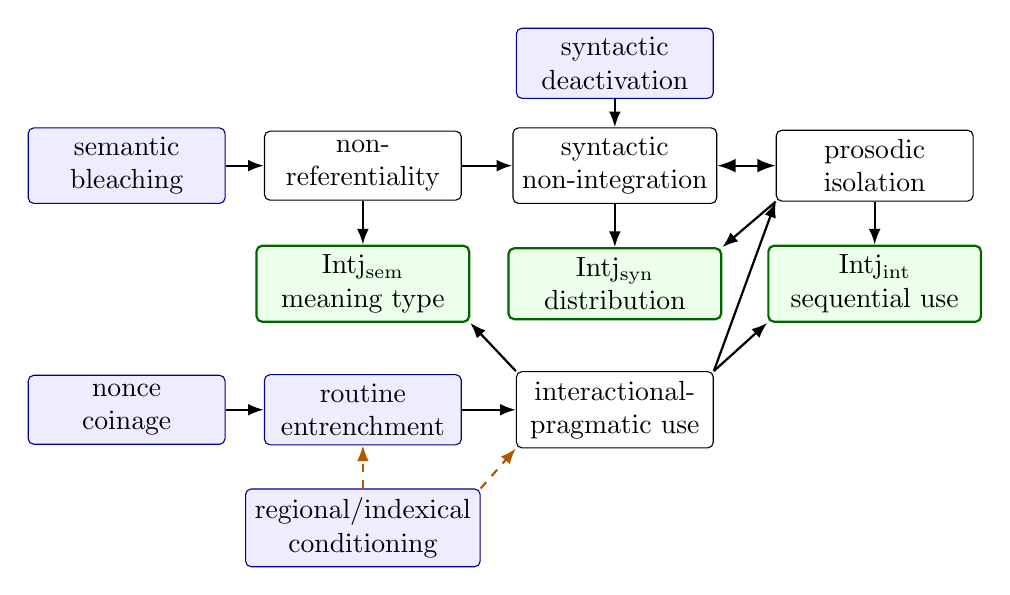
\begin{tikzpicture}[
  node distance=9mm and 12mm,
  process/.style={
    draw,
    rounded corners=2pt,
    align=center,
    draw=blue!55!black,
    fill=blue!7,
    minimum width=25mm,
    minimum height=8mm
  },
  property/.style={
    draw,
    rounded corners=2pt,
    align=center,
    fill=white,
    minimum width=25mm,
    minimum height=8mm
  },
  field/.style={
    draw,
    thick,
    rounded corners=2pt,
    align=center,
    draw=green!40!black,
    fill=green!8,
    minimum width=27mm,
    minimum height=9mm
  },
  arrow/.style={-{Latex[length=2mm]}, thick},
  mutual/.style={<->, >=Latex, thick},
  candidate/.style={-{Latex[length=2mm]}, thick, dashed, draw=orange!70!black}
]

\node[process] (bleach) at (0, 2.4) {semantic\\bleaching};
\node[property] (nonref) at (3.0, 2.4) {non-\\referentiality};
\node[property] (synt) at (6.2, 2.4) {syntactic\\non-integration};
\node[property] (pros) at (9.5, 2.4) {prosodic\\isolation};

\node[process] (deact) at (6.2, 3.7) {syntactic\\deactivation};
\node[process] (coinage) at (0, -0.7) {nonce\\coinage};
\node[process] (routine) at (3.0, -0.7) {routine\\entrenchment};
\node[property] (intuse) at (6.2, -0.7) {interactional-\\pragmatic use};
\node[process] (social) at (3.0, -2.2) {regional/indexical\\conditioning};

\node[field] (semnode) at (3.0, 0.9) {Intj\textsubscript{sem}\\meaning type};
\node[field] (synnode) at (6.2, 0.9) {Intj\textsubscript{syn}\\distribution};
\node[field] (intnode) at (9.5, 0.9) {Intj\textsubscript{int}\\sequential use};

\draw[arrow] (bleach) -- (nonref);
\draw[arrow] (nonref) -- (synt);
\draw[mutual] (synt) -- (pros);
\draw[arrow] (deact.south) -- (synt.north);
\draw[arrow] (coinage) -- (routine);
\draw[arrow] (routine) -- (intuse);
\draw[arrow] (intuse.north east) -- (pros.south west);
\draw[candidate] (social) -- (routine);
\draw[candidate] (social.north east) -- (intuse.south west);

\draw[arrow] (nonref.south) -- (semnode.north);
\draw[arrow] (intuse.north west) -- (semnode.south east);
\draw[arrow] (synt.south) -- (synnode.north);
\draw[arrow] (pros.south west) -- (synnode.north east);
\draw[arrow] (intuse.north east) -- (intnode.south west);
\draw[arrow] (pros.south) -- (intnode.north);

\end{tikzpicture}%
}
\caption{Schematic causal-pragmatic network for English interjections.
Blue nodes mark recruitment, ordering, or stabilizing processes; white
nodes mark diagnostics; and green nodes mark field-relative interjection
nodes. Solid arrows indicate proposed ordering links. The double arrow
marks reciprocal prosodic-syntactic coupling. Dashed orange arrows mark
the regional/indexical maintenance hypothesis. The three field-relative
nodes overlap in extension but support different predictions.}
\label{fig:causal-network}
\end{figure}

\subsection{Causal residues at the category boundary}\label{sec:residues}

The interjection cluster is a convergence point, but convergence doesn't
erase history. Forms recruited through different pathways can share the
same pragmatic profile while retaining traces of the source construction
that brought them there. Those traces explain why the category is both
recognizable and persistently irregular. The irregularities are pathway
signatures rather than noise around a prototype.

This gives the category a second kind of inference. Section~\ref{sec:projectibility}
develops forward projectibility: observing some properties of a novel
form licenses predictions about other properties. Historical pragmatics
also needs a \term{retrodictive counterpart to projectibility}:
observing a residual property can license an inference about the pathway
that produced it. A causal-network account can make that inference
because it links properties to recruitment pathways, ordering relations,
and source constructions.

Table~\ref{tab:pathway-residues} collects the residues each recruitment
pathway leaves behind, and the retrodictive inference each one licenses.

\begin{table}[t]
\centering
\small
\caption{Pathway residues in the English interjection cluster}
\label{tab:pathway-residues}
\begin{tabular}{@{}
  >{\raggedright\arraybackslash}p{.20\textwidth}
  >{\raggedright\arraybackslash}p{.18\textwidth}
  >{\raggedright\arraybackslash}p{.27\textwidth}
  >{\raggedright\arraybackslash}p{.25\textwidth}
  @{}}
\toprule
Pathway & Gateway & Residue & Retrodictive prediction \\
\midrule
Religious noun or proper name & Vocative invocation &
Taboo avoidance, euphemistic phonological divergence, loss of reference
without complement residue (\mention{Jesus!}~$>$~\mention{jeez},
\mention{gee}; \mention{God!}~$>$~\mention{gosh}, \mention{golly}) &
Euphemistic deformation plus no argument structure points to an
invocative source. \\
\addlinespace
Verb or imperative & Directive or imperative frame &
Complement residue, second-person orientation, directive force, particle
retention (\mention{damn these mosquitoes!}, \mention{come on},
\mention{look}) &
An NP complement or directive orientation points to a verbal or deontic
source. \\
\addlinespace
Onomatopoeic or interactional coinage & Iconic or interactional vocalization &
Atypical phonology, reduplication, spelling variation, weak etymological
transparency (\mention{ugh}, \mention{whew}, \mention{tut-tut},
\mention{uh-oh}, \mention{shh}) &
Noncanonical phonology without a plausible lexical source points to
iconic coinage. \\
\addlinespace
Interactional recruitment or regional/indexical conditioning & Sequential slot or community marker &
Regional skew, register sensitivity, indexical persistence
(\mention{lah}, \mention{yaar}, \mention{haba}, \mention{bruh},
\mention{mm-hm}) &
Uneven distribution by community points to regional/indexical
entrenchment or conditioning. \\
\bottomrule
\end{tabular}
\end{table}

The residue analysis turns apparent exceptions into evidence. \mention{Damn these
mosquitoes!} becomes a verbal-path residue rather than an anomalous
interjection with a complement. \mention{Gee} records taboo-managed
invocative recruitment through euphemistic phonology. \mention{Lah}
looks like the kind of item expected if regional or indexical
conditioning stabilizes some interjectional forms. Prototype theory
predicts fuzzy boundaries.
It doesn't predict that different boundary failures should line up with
different historical routes.

The same logic applies when forms leave the cluster. A pre-registered
COHA check of verbal derivatives shows that early VP-head uses of
\mention{wowed}, \mention{booed}, \mention{oohed}, and
\mention{shooed} retain source-interjection semantics after syntactic
integration (Appendix~\ref{app:morphgain}).%
\footnote{The analysis plan was committed before extraction and coding
  (\texttt{f1a2193}, 27 May 2026). \ifblind The full pre-registration,
  data, and code are archived at [link removed for blind review].\else
  The full pre-registration, data, and code are archived at
  \url{https://github.com/BrettRey/interjections-hpc}.\fi}
These exit cases fit the residue account: syntactic integration removes
\term{interjection\textsubscript{syn}}, while source-interjection semantics
persists. They probe boundary behaviour, not corrective control.

The \mention{fie} study marks the limit of residue reasoning under
global attrition. The pre-registered prediction was that
\term{interjection\textsubscript{int}} would weaken before
\term{interjection\textsubscript{sem}}, and \term{interjection\textsubscript{sem}}
before \term{interjection\textsubscript{syn}}. In COHA, all three node
diagnostics decline together (Appendix~\ref{app:fie}).%
\footnote{The analysis plan was committed before data extraction
  (\texttt{e18675b}, 15 March 2026). \ifblind The full
  pre-registration, data, and code are archived at [link removed for
  blind review].\else The full pre-registration, data, and code are
  archived at \url{https://github.com/BrettRey/interjections-hpc}.\fi}

When a community stops actively using a form, evidence for the pathway
can disappear across nodes at once. The relevant process is loss of the
ecology in which the ordering links operate, not pathway-specific property
loss. Interjections remember how they got there, and those residues make
the category's boundary behaviour structured rather than accidental.

\subsection{Stability through turnover}\label{sec:turnover}

Pathway residues show that interjectional forms remember how they entered
the network. Turnover shows the complementary fact: the interjection
profile can remain available while its lexical inventory changes.
Individual forms enter and leave, but the broad profile remains
available for new material.

The Corpus of Historical American English (COHA) illustrates this
turnover. Among words tagged as interjections, \mention{nay} ranks in
the top~10 in the 1820s but falls to negligible frequency by the 2010s;
\mention{yeah}, entirely absent from the 1820s data, is among the five
most frequent interjection-tagged forms by the 2010s.%
\footnote{Based on part-of-speech--tagged frequencies in COHA \citep{davies2010}.
  Frequencies are normalized per million words. The interjection tag
  captures a conventional inventory rather than a theoretically motivated
  one; the point here is the turnover pattern, not the tagging decisions.}
The items change while the projectible category position remains
available.

Regional variation shows the profile's availability under different
local inventories.
The GloWbE corpus \citep[1.9~billion words across 20 English-speaking
countries]{daviesfuchs2015} shows that candidate interjectional forms
are distributed unevenly across varieties, with \mention{lah} almost
exclusively in Singapore and Malaysia, \mention{yaar} in India and
Pakistan, and \mention{haba} in Nigeria. The corpus evidence establishes
distributional conditioning; the linguistic analysis identifies the
shared profile that makes those forms comparable.

The cluster is also continuously replenished via onomatopoeia. Nonce
interjections can be freely coined \citep[74]{quirk1985}, and new coinages
immediately adopt the cluster profile: they're prosodically isolated,
non-referential, emotively laden, and syntactically non-integrated.

This generates a testable prediction: a newly conventionalized
interjectional use should exhibit the full cluster profile without
having traversed the documented noun-to-interjection or
verb-to-interjection paths. Standalone interjectional uses of recent
forms like \mention{bruh}, \mention{yeet}, and \mention{oof} fit this
expectation, since those uses are prosodically isolated, non-inflecting,
non-referential, and syntactically non-integrated, even when the same
word families include verbal or nominal lexemes. The category position remains
available even as its members turn over.

\textcite{dingemanse2020} characterizes such items as \term{liminal signs},
signs at the boundary between sound and speech, whose liminality is
functional, not defective. Cultural evolutionary processes \enquote{sample
the landscape of possible resources} \citep[191]{dingemanse2020}. The
causal-network account describes that landscape as a property space
structured by the recruitment pathways and synchronic links above.

The recruited, ordered, and replenished cluster is now ready for the
paper's central inferential question: what can partial evidence license?

\section[Projectibility]{Projectibility: what the category lets you predict}\label{sec:projectibility}

Section~\ref{sec:cluster} showed what each property, individually, lets
you infer. Section~\ref{sec:causal-structure} identified the ordering
and stabilizing links that couple those properties. This section asks a
different question: what does the package license, and for whom?
Section~\ref{sec:residues}
treated retrodictive inference from residue to recruitment history; here
\term{projectibility} means forward inference from observed properties of
a form to properties not yet observed.

That formulation matters for the question of \emph{whose} inference is at
issue. Speakers and hearers use partial cues to anticipate how a form will
behave before they've observed its full distribution, and they do so without
holding the category label; analysts run the same inference explicitly, from
category membership, for field-specific purposes.
Section~\ref{sec:proj-partial} separates the two.

The paper's central claim is that interjections are a
\term{causal-pragmatic kind} whose richest
projectibility concerns stance expression, interactional-pragmatic
distribution, and conversational management rather than
truth-conditional denotation. The section first shows how partial
observations support participant inference, then shows how the same
structure yields different predictions for syntax, semantics, and
interactional pragmatics. From here on, bare \enquote{interjection}
refers to the zone where the three field-relative nodes overlap unless a
subscript specifies otherwise.

The running case is the word family \mention{damn}. Standalone
interjectional \mention{damn!}, complement-taking \mention{damn these
mosquitoes!}, and prenominal \mention{damn} in \mention{the damn car}
belong to the same word family. They needn't share a lexeme.
That contrast makes the methodological point concrete: the network
classifies lexical items in grammatical environments, not word families.

\subsection{Partial-observation inference}\label{sec:proj-partial}

Projectibility becomes circular if it says only this: if X is an
interjection, it has interjection properties. That's trivially true of
any category. Causal-network projectibility is different. Observing some
cluster properties in a novel form licenses inference to other
properties you haven't yet observed.

Consider the standalone interjectional use of \mention{bruh}, a
recently conventionalized form. A learner or hearer encountering that
use for the first time observes a partial package: standalone position,
prosodic isolation, morphological bareness, and stance meaning. From
those observations, the three field-relative nodes license a battery of
further expectations:

\ea\label{ex:bruh}
  \ea \term{interjection\textsubscript{syn}}: the interjectional use
    won't inflect within that use (*\mention{bruhs}, *\mention{bruhed}),
    will resist syntactic integration (*\mention{I think that bruh,
    we're late}), and won't take a determiner or function as an argument
    (*\mention{the bruh}, *\mention{Bruh surprised me}). This leaves
    room for separate nominal or verbal lexemes in the same word family.
  \ex \term{interjection\textsubscript{int}}: the form should be available for
    turn-initial or standalone interactional use.
  \ex \term{interjection\textsubscript{sem}}: its expressive meaning is
    expected to be use-conditional and speaker-oriented.
  \z
\z
These expectations vary in strength, and the asymmetry matters:

\begin{itemize}
\item Near-entailments (a): the
  \term{interjection\textsubscript{syn}} predictions mostly extrapolate
  within the same domain from observed distributional facts. Any
  framework recognizing the relevant morphosyntactic properties
  generates many of the same predictions. These are real but not specific
  to the causal-network account.
\item Cross-domain inferences (b, c): the
  \term{interjection\textsubscript{int}} prediction (interactional-pragmatic
  distribution from phonological form) and the
  \term{interjection\textsubscript{sem}} prediction (use-conditional meaning
  from stance expression) involve genuine leaps across linguistic
  levels. These are specific to the causal-network account: they rely on
  the cluster's internal links, not on any single property.
\end{itemize}
All three are licensed because identifiable links order the cluster's
properties. The non-referentiality ratchet
(Section~\ref{sec:synchronic-coupling}) links loss of referential content with
syntactic non-integration. Prosodic-syntactic coupling then links
syntactic non-integration with prosodic isolation. The inferences are
grounded in network order, not in definitions.

Who does the projecting, though? A hearer meeting \mention{Bummer!} or
\mention{groovy} for the first time doesn't run a taxonomy and then read
off consequences. So it's worth separating two levels that the argument so
far has run together.

\term{Category-driven projection} is the analyst's. Given that a form
belongs to the interjection cluster, expect the linked properties. That's
projectibility in Goodman's sense, and it's what the preceding sections
have claimed. \term{Cue-driven inference} is the participant's. The
\mention{bruh} case above describes it without naming it: what the hearer
has is standalone position, prosodic isolation, morphological bareness, and
stance meaning, and the stance reading follows from those. No category
label need be represented for the reading to go through.

The two aren't rivals, and the relation between them matters for the
account. Cue-driven inference is reliable \emph{because} the cluster is
coupled: the links in Section~\ref{sec:synchronic-coupling} are what make a
partial package informative about the rest. Analyst and participant are two
consumers of one causal structure, drawing on it for different purposes and
with different explicitness. So \mention{Bummer!} and \mention{groovy} tell
against an account on which the category label does the inferential work,
and for one on which the coupling does. The label is the analyst's
bookkeeping device for a structure participants exploit without naming.

Fields differ in which links they track
(Section~\ref{sec:proj-fieldrelative}); analyst and participant differ in
whether the category figures in the inference at all. The two indices are
independent. Nothing here says that speakers tacitly represent
interjection-hood, and the account doesn't need them to.

\subsection{Field-relative projectibility}\label{sec:proj-fieldrelative}

Different fields track categories with roughly the same extension but
different causal links and different inferential payoffs. That
field-relativity follows from treating kinds as nodes in causal
structures: a field tracks the node whose causal relations support its
explanations and predictions.
The three interjection nodes introduced in
Section~\ref{sec:fieldrelative-nodes} do their work as different
packages of inference, not as rival definitions.

\term{interjection\textsubscript{syn}} projects syntactic behaviour:
supplement function, resistance to \mention{that}-complementation,
resistance to coordination with non-interjections, and no ordinary
argument structure. These predictions are grounded in the
prosodic-syntactic coupling link from
Section~\ref{sec:synchronic-coupling}. \term{interjection\textsubscript{sem}}
projects meaning type: use-conditional contribution,
speaker-oriented attitude, nondisplaceability, and descriptive
ineffability \citep[166]{potts2007}. I treat these as a cluster linked
by semantic bleaching, rather than as a stipulative definition of
\textcite{potts2007}'s \term{expressives}. \term{interjection\textsubscript{int}}
projects interactional-pragmatic behaviour: turn-initial or standalone
positioning, independent intonation contour, stance display, and
availability for backchanneling. These predictions are grounded in
routine entrenchment and possibly in regional/indexical conditioning
\citep{stivers2019,dingemanse2020}.

The nodes overlap because some links, especially prosodic isolation
and non-referentiality, contribute to more than one node. They come
apart because other links are field-specific. A novel form categorized
as \term{interjection\textsubscript{syn}} (prosodically isolated,
non-inflecting, syntactically non-integrated) should tend also to be
\term{interjection\textsubscript{sem}} (use-conditional, speaker-oriented)
and \term{interjection\textsubscript{int}} (turn-initial, available for
backchanneling). Central cases such as \mention{wow}, \mention{ouch},
and \mention{hey} fit that default. Boundary cases locate the
decoupling: \mention{mm-hm} is \term{interjection\textsubscript{int}} but
debatably \term{interjection\textsubscript{syn}} \citep{oconnell2005}.

The three constructions of \mention{damn} show the same point inside a
single word family.

For standalone
\mention{damn!}, all three nodes agree: the form is prosodically
isolated, syntactically non-integrated, use-conditional, and available
as a stance marker. For \mention{damn these mosquitoes!}, the picture
is mixed: \term{interjection\textsubscript{syn}} holds (it heads an IntjP)
but with limited complement-taking;
\term{interjection\textsubscript{sem}} holds (the meaning is expressive);
\term{interjection\textsubscript{int}} is weakened (it's not a backchannel or
turn-management device).

For prenominal \mention{damn} in \mention{the damn car}, the nodes
diverge further: \term{interjection\textsubscript{syn}} fails entirely (the
form is syntactically integrated inside a noun phrase), but
\term{interjection\textsubscript{sem}} holds (use-conditional, perspective-
dependent). Neither \textit{CGEL}'s syntax nor Potts's semantics alone
predicts this gradient. The three-node analysis does, because it tracks
which links are active in each construction.

\subsection{Category vs.\ function}

\textit{CGEL}'s distinction between category and function sharpens the
projectibility point: what does the \term{interjection\textsubscript{syn}} category label add
beyond the \term{supplement} function label? Supplements of any category
(noun phrases [NPs], adjective phrases [AdjPs], relative clauses) share
prosodic isolation and syntactic
non-integration. But \term{interjection\textsubscript{syn}} adds a package of
predictions that no other category-in-supplement-function supports:

\begin{itemize}
\item Non-referentiality. Supplements can be referential
  (\mention{a university professor, Dr.~Brown, \ldots}); interjections
  characteristically can't.
\item Emotive/interpersonal force. Not all supplements express
  stance; interjections characteristically do.
\item Free coinage. No other category in supplement function
  can be freely coined via onomatopoeia.
\item Non-inflection. NP supplements inflect freely;
  interjections don't.
\end{itemize}

The function label tells you about syntactic integration. The category
label tells you about inference: it licenses a package of predictions
that the function label alone can't provide. The category/function distinction matters
beyond the \textit{CGEL} tradition: any framework that distinguishes what kind of
thing an expression is from what job it's doing in a particular clause
will face the same question. The causal-network answer is that the
category earns its keep by licensing inferences that the function
doesn't.

\subsection{Interjections as a causal-pragmatic kind}\label{sec:proj-pragmatic}

The three-node analysis explains why interjections are centrally
pragmatic. Not all categories project in the same domain. Nouns project
morphosyntactically: they take determiners, inflect for number, fill
argument slots. Categorizing something as a noun tells you almost
nothing about its pragmatics, since nouns aren't a pragmatic category.

For interjections, the situation is reversed. The three nodes overlap,
and the richest projectibility belongs to
\term{interjection\textsubscript{int}}, the interactional-pragmatic
cluster.
\textcite{dingemanse2024} reaches the same conclusion from interactional
data: the most frequent and functionally central interjections are
interactional tools (continuers, repair initiators, change-of-state
tokens) rather than emotive exclamations, and their primary
projectibility is about sequential position and conversational
management. The forms at the intersection of all three nodes are a
\term{causal-pragmatic kind}: their strongest inferences are about use,
not denotation.

Why pragmatic? Because causal links generate predictions within the
domains they operate in. The prosodic-syntactic coupling from
Section~\ref{sec:synchronic-coupling}
predicts prosodic and syntactic behaviour, with no corresponding
prediction about morphological paradigms or truth-conditional content.
Regional/indexical conditioning predicts uneven persistence across
varieties, with no corresponding prediction about inflectional
regularity. The strongest established links among the three
interjection nodes are prosodic and interactional; the regional or
indexical link remains a maintenance hypothesis. These links and
hypotheses underwrite predictions in their respective domains.

The same point holds outside interjections. Noun projectibility is
morphosyntactic because the underlying processes (agreement, structural
analogy, discourse frequency) operate in morphosyntactic domains.

This connects to the content/procedural distinction. The central
projectibility of interjections is procedural and use-conditional rather
than denotational \citep{TraugottDasher2002}. The
\term{interjection\textsubscript{sem}} (expressive) cluster is the semantic
reflex: use-conditional meaning is the semantic signature of procedural
content. The parallel with other domain-specific kinds supports the
pattern. \term{Animacy} projects grammatically (argument realization,
reference tracking); \term{colour} projects ecologically (edibility,
toxicity) but usually doesn't project grammatically in the way animacy
can \citep[cf.][]{seifart2010}. In each case, the domain of
projectibility follows from the underlying processes.

The richest projectibility is pragmatic, but
\term{interjection\textsubscript{syn}} still belongs in the grammar
because it's projectible and has its own causal links. Neutralize
prosodic isolation and the form is reclassified. The syntactic category
licenses distributional inference: it predicts supplement function,
embedding resistance, and coordination
restrictions, even if those predictions are less rich than the
pragmatic ones. A thin syntactic node is still a projectible syntactic
node. The framework requires reliable inference, and
\term{interjection\textsubscript{syn}} does.

\section{Discussion}\label{sec:discussion}

\subsection{Empirical probes and boundary conditions}

Section~\ref{sec:projectibility} asked what categorizing a novel form as
an interjection lets you predict about that form. At the category level,
the causal-network account should also explain patterns across the
interjectional region as a whole. Prototype theory accommodates graded
membership, fuzzy boundaries, and better-and-worse exemplars
\citep{rosch1975}. The causal-network account adds
network-order predictions with named defeat conditions. The probes
below address stable profiles, boundary behaviour, and failure. They
aren't tests of corrective control.

The strongest probe is pathway residue. If interjections are recruited by
different causal pathways, residual properties should line up with
recruitment history. The defeat condition is random distribution:
retained complements, euphemistic deformation, atypical phonology, and
regional skew should show no relation to source pathways. The evidence
in Section~\ref{sec:residues} supports the residue prediction, and the
pre-registered morphology-gain study adds an exit-residue case:
\mention{wowed}, \mention{booed}, \mention{oohed}, and \mention{shooed}
gain syntactic integration while retaining source-interjection semantics.
The payoff is pragmatic and diachronic: boundary failures diagnose
recruitment routes and explain why later uses keep source-specific
residues.

A second probe asks whether conditioning recovers structure. Apparent
gradation at the interjection boundary should decompose when conditioned
on register, dialect, or community. The defeat condition is parity
between conditioned and pooled models. A proof-of-concept probe uses
GloWbE frequency data \citep{daviesfuchs2015}: for the 10 most frequent
interjection-tagged items plus regional and boundary items,
frequency-per-million was extracted by country (20 countries) by raw
string search, and the coefficient of variation (CV; standard deviation
divided by the mean) was computed across countries.

The results show three tiers of geographic conditioning. Regional
interjections (\mention{lah}, \mention{yaar}, \mention{haba}) are
near-categorical: \mention{lah} occurs at 9.35 per million in Malaysia
and 6.72 in Singapore but near zero elsewhere; \mention{yaar} at 2.88
in Pakistan and 2.33 in India but near zero elsewhere; \mention{haba}
at 8.78 in Nigeria but near zero elsewhere.

Core interjections show
intermediate but structured variation: \mention{ah} has the highest
CV among core items (0.71), with Singapore (60.42) and Jamaica (53.16)
at eight times the rate of Kenya (7.62). Even broadly distributed items
like \mention{yeah} (CV 0.55) show a 6:1 ratio between the United
States (103.78) and Tanzania (16.85). Only \mention{yes} and
\mention{no} approach uniformity (CVs of 0.21--0.22). Boundary items
continue the pattern: the fillers \mention{um} (CV 0.61) and
\mention{uh} (CV 0.76) and the routine formula \mention{bye} (CV 0.61)
all show structured geographic variation.

Conditioning on country recovers structure at every level of this
sample. Variety structures the apparent gradience between core
interjections, fillers, and boundary items.

A Bayesian multilevel model (negative binomial with crossed random
effects for item and country) supports the same point. Adding country as
a grouping factor improves prediction over an item-only baseline: the
country-level random-effect standard deviation is 0.44 (95\% credible
interval [CrI]: 0.28--0.65), and the conditioned model outperforms the
unconditional model by 18 expected log predictive density (ELPD) units
(standard error [SE] 13) on exact leave-one-out cross-validation.

The descriptive CV results are the primary evidence; the model shows
that the pattern survives a crossed random-effects structure. Full model
specification and results are in the
supplementary materials.\footnote{\ifblind Available at
  [link removed for blind review].\else Available at
  \url{https://github.com/BrettRey/interjections-hpc}.\fi}
Several methodological limitations remain. GloWbE's
part-of-speech tagger, trained on inner-circle English, fails to tag
regional interjections (\mention{yaar} and \mention{haba} receive no
interjection tag at all), which means the tagged frequencies
underestimate regional items. The \mention{ha} data is noisy
because the tagger captures laughter representations
(\mention{HA! HA!}) alongside genuine interjection uses.

Country differences in GloWbE may also reflect corpus composition,
genre mix, internet ecology, and orthographic convention as much as
dialect or community structure. Raw strings are imperfect proxies too:
\mention{yes}, \mention{no}, \mention{ha}, \mention{ah},
\mention{oh}, \mention{well}, \mention{right}, and \mention{like} are
not automatically interjection tokens. Some are clausal, quoted,
discourse-marker uses, literary representations, or noise. The
methodological payoff is that conditioning by variety reveals structure
that pooled category labels hide.

A third, weaker probe concerns hub-property asymmetry. One property may
be more central to network order than others, with prosodic isolation
and non-referentiality as the main candidates. The defeat condition is
equal contribution by all properties. The present evidence leaves this
prediction open.

Onomatopoeic interjections like \mention{pop} can be
syntactically integrated into clause structure; when prosodic isolation
is neutralized, as when \mention{pop} in \mention{pop went the cork}
is an adverb rather than a standalone interjection
\citep[152]{meinard2015}, reclassification is immediate. Restoring
partial referentiality, by contrast, allows the form to hover between
noun and interjection uses (as with \mention{God}). This suggests
prosodic isolation may be the hub, but the evidence is indirect.

The probes differ in evidential weight. Pathway residue is the main
explanatory payoff, conditioning by variety is a proof of concept, and
hub-property asymmetry is an open conjecture. Prototype theory describes
the gradience but doesn't predict the trajectory of entry, the
pathway-specific structure of boundary cases, or the structure hidden in
apparent variation.

At the framework level, if a feature-based account
(e.g., [\textsc{+peripheral}, \textsc{-argument-taking},
\textsc{+expressive}]) generates the same predictions without causal
structure, the network account would be a relabelling. The
causal-network payoffs are pathway residues and the field-relative
decomposition; if both fail under further testing, the case for
interjections as a causal-pragmatic kind collapses to a descriptive
property list.

\subsection{Interjections as a thin causal-pragmatic kind}

\term{interjection\textsubscript{syn}} is thin compared with the
corresponding noun and verb nodes. It lacks the dense network of
agreement, argument realization, derivation, and inflectional behaviour
that makes those categories so stable. Thin syntax still licenses
inference. The syntactic node predicts supplement function, embedding
resistance, coordination restrictions, and non-argumenthood.

The category is richest where three nodes intersect. The syntactic node
supplies distributional projectibility; the semantic node supplies
use-conditional and expressive projectibility; and the interactional
node supplies sequential and interactional projectibility. Interjections
are thin as a syntactic category and rich as a causal-pragmatic kind.

\subsection{Boundary disputes as causal-link overlap}\label{sec:boundaries}

The graded boundaries that embarrassed classical category theory
(interjections vs.\ nouns, verbs, adverbs, fillers, routine formulae)
are field-relative predictions of the causal-network account. Each
boundary reflects partial causal-link overlap and differences in what a
field needs the category to predict.

Routine formulae (\mention{bye}, \mention{hello}, \mention{sorry}) share
prosodic isolation and pragmatic function with interjections but add
addressee-directedness and social predictability
\citep[109--110]{ameka1992}. For grammar, those shared properties place
them near interjections. For speech-act analysis, the additional
properties matter more, because they predict conventional response slots,
addressees, and felicity conditions. They're structured by additional
processes (social convention, politeness norms) that prototypical
interjections don't require.

Fillers (\mention{um}, \mention{uh}) share prosodic distinctiveness and
syntactic non-integration but differ in emphasis, pause distribution,
and citation-introduction ability \citep{oconnell2005}. They occupy a
neighbouring region of the property space, structured by partially
overlapping links (processing-pressure management rather than
emotive expression).

The Ameka-Wilkins debate can be reframed in these terms. Ameka's
separation is right for a field that needs to predict social routines and
speech-act felicity \citep[109]{ameka1992}. Wilkins's inclusion is right
for a field that needs to track pragmatic and semantic overlap with
interjections \citep[142]{wilkins1992}. A causal-network account accommodates both
observations because projectibility is indexed to explanatory purpose.

\section{Conclusion}\label{sec:conclusion}

English interjections are a category whose members support projectible
inferences about use. Assigning a form to it lets an analyst predict
prosodic packaging, supplement function, use-conditional stance,
sequential position, response function, and uptake, and the coupling that
licenses those predictions is what lets speakers and hearers anticipate the
same behaviour from partial cues. The category is thin as syntax but rich
as pragmatics.

The reason is that the familiar interjection profile is a stable
causal-pragmatic cluster. Diachronic pathways recruit forms into the
profile: grammaticalization via semantic bleaching, pragmaticalization
via syntactic deactivation, and nonce coinage via onomatopoeia.
Synchronic links then structure the profile: prosodic-syntactic
coupling, the non-referentiality ratchet, interactional routine
entrenchment, and possibly regional/indexical conditioning. These links
explain why partial observations support further inferences.

The field-relative decomposition
(\term{interjection\textsubscript{syn}},
\term{interjection\textsubscript{sem}}, and
\term{interjection\textsubscript{int}}) shows why the traditional label
is useful but not uniform. Syntax, semantics, and interactional
pragmatics track overlapping nodes with different predictive payoffs.
Boundary cases such as \mention{damn these mosquitoes!}, prenominal
\mention{damn}, fillers, routine formulae, and obsolete \mention{fie}
aren't embarrassing exceptions; they show which links are active and
which have weakened.

The broader pragmatic payoff is path dependence. Interjections don't
merely express emotion; they enter utterances with histories that shape
stance, sequence, and uptake. \mention{Gee}, \mention{damn},
\mention{bruh}, \mention{wowed}, and \mention{fie} matter because they
show projectible profiles, boundary behaviour, exit residues, and
failure conditions. They show how a fuzzy category can support pragmatic
inference without a classical essence.

The evidence establishes projection targets, a stable profile, network
order, and maintenance hypotheses. It doesn't establish strict
homeostatic control. That limit matters: pragmatic categories can be
stable and inductively useful without being maintained by a
perturbation-sensitive control system. English interjections are one
such category.

\ifblind\else
\section*{Acknowledgements}

I compiled empirical material for the Wikipedia article
\enquote{English interjections}, of which I'm the primary author. This
paper reanalyses that material through the lens of pragmatic
projectibility.

Supplementary materials (data and analysis code for the corpus tests)
are available at
\url{https://github.com/BrettRey/interjections-hpc}.
\fi

% AI disclosure moved to page 1 via \aidisclosure{} after the keywords,
% per house style from 2026-07-16. The end-of-paper Elsevier-form
% declaration that stood here has been removed to avoid duplication.

\clearpage
\begingroup
\setlength{\emergencystretch}{3em}
\printbibliography
\endgroup

\clearpage
\appendix
\section[Supplementary materials]{Supplementary materials: GloWbE conditioning analysis}
\label{app:conditioning}

\subsection{Data}

Frequency counts for 18 items were extracted from the GloWbE corpus
\citep{daviesfuchs2015}: 1.9 billion words across 20 countries. Items
include the 10 most frequent interjection-tagged forms (\mention{yes},
\mention{no}, \mention{oh}, \mention{yeah}, \mention{hi}, \mention{hey},
\mention{wow}, \mention{hello}, \mention{ah}, \mention{ha}), three
regional interjections (\mention{lah}, \mention{yaar}, \mention{haba}),
the semi-regional \mention{eh}, the boundary items \mention{cheers} and
\mention{bye}, and the fillers \mention{um} and \mention{uh}.

Figure~\ref{fig:country-variation} displays raw frequency per million
words by country for each item.

\begin{figure}[ht]
  \centering
  
\includegraphics[width=\textwidth]{country-variation.pdf}
  \caption{Interjection frequency per million words across 20 GloWbE
    countries. Red points indicate the median across items within each
    country. Regional items (\mention{lah}, \mention{yaar},
    \mention{haba}) cluster in one or two countries. Core items show
    structured cross-country variation. Only \mention{yes} and
    \mention{no} approach uniformity.}
  \label{fig:country-variation}
\end{figure}

\subsection{Model specification}

Four Bayesian negative binomial models were fitted using
\texttt{brms}~2.23 in R, with 4 chains of 2{,}000 iterations (1{,}000
warmup) each. The confirmatory models (m0--m2) use exact reloo for
leave-one-out cross-validation; the exploratory model (m3) is assessed
by Pareto-smoothed importance sampling (PSIS) diagnostics only.

\begin{quote}
\small
\noindent\texttt{m0} (unconditional):\\
\texttt{count \textasciitilde{} 1 + offset(log(words\_m)) + (1~|~item)}

\noindent\texttt{m1} (conditioned):\\
\texttt{count \textasciitilde{} 1 + offset(log(words\_m)) +}\\
\texttt{(1~|~item) + (1~|~country)}

\noindent\texttt{m2} (item type):\\
\texttt{count \textasciitilde{} 1 + item\_type + offset(log(words\_m)) +}\\
\texttt{(1~|~item) + (1~|~country)}

\noindent\texttt{m3} (exploratory):\\
\texttt{count \textasciitilde{} 1 + item\_type + offset(log(words\_m)) +}\\
\texttt{(1~|~item) + (1~+~item\_type~||~country)}
\end{quote}

Model m3 estimates country-level varying slopes by item type. Because
several item-type cells are sparse (semi-regional: 1 item, boundary: 2,
filler: 2, regional: 3), these slopes are thinly supported and m3 is
treated as exploratory.

\subsection{Results}

Exact leave-one-out cross-validation (confirmatory models):

\begin{center}
\begin{tabular}{lrr}
  \hline
  Model & ELPD diff & SE diff \\
  \hline
  m1 (conditioned) & 0.0 & 0.0 \\
  m2 (item type) & $-$9.3 & 7.9 \\
  m0 (unconditional) & $-$17.9 & 13.3 \\
  \hline
\end{tabular}
\end{center}

The conditioned model (m1) is preferred. Adding item-type fixed effects
(m2) doesn't improve on m1 because the item random effect already
captures between-item variation. The exploratory model (m3) is excluded
from formal ranking because 9 observations retain Pareto $k > 0.7$
after moment matching, indicating unstable PSIS leave-one-out estimates.

Random effects from the conditioned model (m1):
\begin{itemize}
  \item Country standard deviation (SD) = 0.44 (95\% CrI: 0.28--0.65)
  \item Item SD = 2.07 (95\% CrI: 1.49--2.96)
  \item Ratio: 4.7:1 (item identity explains more variation, while
    country adds structure)
\end{itemize}

The evidence is directionally consistent: conditioning on country
improves prediction ($\Delta$ELPD = 17.9, SE 13.3), and the country
random-effect SD is positive across the interval. The SE is large
relative to the point estimate, reflecting the small sample (18 items $\times$ 20
countries = 360 observations). The descriptive CV results in the main
text provide the primary evidence for the conditioning probe; the model
suggests the pattern survives the crossed random-effects structure.

\section[Morphology gain in COHA]{Supplementary materials: morphology-gain analysis (COHA)}
\label{app:morphgain}

\subsection{Data and extraction}

The morphology-gain study was pre-registered before extraction and
coding (\texttt{f1a2193}, 27 May 2026). The corpus was COHA
(1820--2019). The fixed source families were \mention{wow},
\mention{boo}, \mention{ooh}, and \mention{shoo}. The fixed target
derivatives were \mention{wowed}, \mention{wowing}, \mention{wows};
\mention{booed}, \mention{booing}, \mention{boos}; \mention{oohed},
\mention{oohing}, \mention{oohs}; and \mention{shooed},
\mention{shooing}, \mention{shoos}. Bare source forms were excluded.

Extraction was completed on 27 May 2026. The token-level analysis used
parsed key-word-in-context (KWIC) exports. Chart requests for
\mention{oohed} and \mention{oohing} returned server errors, but KWIC
exports loaded and were used for coding. Minor chart/KWIC row-count discrepancies are
documented in the extraction summary.

The go/no-go threshold required at least 20 analyzable derivative tokens
and at least two decades with three or more analyzable derivative
tokens. All four families met the threshold.

\begin{center}
\begin{tabular}{lrrl}
  \toprule
  Family & Analyzable tokens & Decades with 3+ & Status \\
  \midrule
  \mention{boo} & 364 & 10 & GO \\
  \mention{ooh} & 52 & 6 & GO \\
  \mention{shoo} & 410 & 13 & GO \\
  \mention{wow} & 143 & 9 & GO \\
  \bottomrule
\end{tabular}
\end{center}

\subsection{Coding}

Each analyzable token was coded for two confirmatory properties. First,
\term{verbal syntax}: whether the derivative heads a VP. Second,
\term{semantic residue}: whether the derivative retains the source
interjection's meaning profile: impressed or evaluative response for
\mention{wow}; disapproval or contempt for \mention{boo}; appreciative
or surprised response for \mention{ooh}; and directive away-sending for
\mention{shoo}.

Two secondary descriptive properties were also coded. \term{Interactional
residue} tracks whether the verbal event retains the source
interjection's social-interactional profile as a recognizable act of
response, uptake, display, or direction. \term{Targeted entity} tracks
whether a target, object, addressee, or stimulus is recoverable. These
secondary codes weren't used in the confirmatory test.

\subsection{Confirmatory result}

For each source family, the confirmatory window was the earliest decade
with at least three analyzable derivative tokens, plus following decades
until the window contained at least ten tokens. The success criterion
was \texttt{verbal\_syntax = 1} and \texttt{semantic\_residue = 1}. The
pre-registered support criterion required the lower bound of the
Jeffreys 95\% interval to exceed 0.5.

\begin{center}
\begin{tabular}{lrlrrl}
  \toprule
  Family & Tokens & Window & $n$ & Successes & Jeffreys 95\% CI \\
  \midrule
  \mention{boo} & 364 & 1920s & 17 & 17 & [0.865, 1.000] \\
  \mention{ooh} & 52 & 1960s--1980s & 10 & 10 & [0.783, 1.000] \\
  \mention{shoo} & 410 & 1890s--1900s & 16 & 16 & [0.857, 1.000] \\
  \mention{wow} & 143 & 1930s--1940s & 11 & 11 & [0.800, 1.000] \\
  \bottomrule
\end{tabular}
\end{center}

All four families support the pre-registered prediction. The secondary
diachronic model wasn't estimated because semantic residue had no
variation among included VP-head tokens.

\subsection{Reliability and files}

A blind 10\% recode was completed ($n=97$, seed 2026). The
confirmatory codes were fully reliable: inclusion, VP-head status, and
semantic residue each had agreement = 1.00 and Cohen's $\kappa = 1.00$.
The secondary descriptive codes were less stable.

\begin{center}
\begin{tabular}{lrr}
  \toprule
  Code & Agreement & Cohen's $\kappa$ \\
  \midrule
  Inclusion & 1.000 & 1.000 \\
  VP-head status & 1.000 & 1.000 \\
  Semantic residue & 1.000 & 1.000 \\
  Interactional residue & 0.887 & 0.297 \\
  Targeted entity & 0.557 & 0.025 \\
  \bottomrule
\end{tabular}
\end{center}

The analysis files are in \path{analysis/morphgain-confirmatory/}. The
main outputs are:

\begin{itemize}
  \item \path{morphgain-extraction-summary.csv}
  \item \path{morphgain-go-nogo-summary.csv}
  \item \path{morphgain-coding-summary.csv}
  \item \path{morphgain-confirmatory-results.csv}
  \item \path{morphgain-earliest-windows.csv}
  \item \path{morphgain-reliability-results.csv}
\end{itemize}

The scripts are:

\begin{itemize}
  \item \path{morphgain-confirmatory-extract.mjs}
  \item \path{morphgain-confirmatory-prepare.py}
  \item \path{morphgain-confirmatory-code-primary.py}
  \item \path{morphgain-confirmatory-analyze.py}
  \item \path{morphgain-confirmatory-reliability.py}
\end{itemize}

\section[Fie in COHA]{Supplementary materials: obsolescence analysis (\mentionhead{fie} in COHA)}
\label{app:fie}

\subsection{Data and coding}

616 tokens of \mention{fie} were extracted from COHA (1820--2019),
excluding 141 optical character recognition (OCR) artefacts (where
\mention{fie} is a
misread of \mention{he}, \mention{the}, or \mention{five}). Each
token was coded for three binary node-membership diagnostics:
syntactic, semantic/use-conditional, and interactional-pragmatic
interjectionhood. These correspond to the \textsubscript{syn},
\textsubscript{sem}, and \textsubscript{int} nodes used above. Coding
criteria are in the pre-registration. The decade column was hidden during
coding.

Intra-coder reliability (10\% blind recode, $n = 62$):

\begin{center}
\begin{tabular}{lrr}
  \hline
  Diagnostic & Agreement & Cohen's $\kappa$ \\
  \hline
  \term{interjection\textsubscript{syn}} & 87.1\% & 0.68 \\
  \term{interjection\textsubscript{sem}} & 96.8\% & 0.90 \\
  \term{interjection\textsubscript{int}} & 96.8\% & 0.90 \\
  \hline
\end{tabular}
\end{center}

\subsection{Raw proportions}

Figure~\ref{fig:fie-raw} shows the proportion of tokens retaining
each diagnostic by decade. All three diagnostics are near ceiling
(85--100\%) through the 1890s, decline sharply between 1900 and 1940,
and fluctuate at low levels thereafter. The late rebounds (1980s,
2000s) reflect historical fiction and Shakespeare adaptations in which
characters use \mention{fie} as a live interjection.

\begin{figure}[ht]
  \centering
  
\includegraphics[width=\textwidth]{fie-raw-proportions.pdf}
  \caption{Proportion of \mention{fie} tokens coded 1 for each
    diagnostic, by decade (COHA, 1820--2019). All three diagnostics
    decline in parallel.}
  \label{fig:fie-raw}
\end{figure}

\subsection{Confirmatory model}

Bayesian logistic decline models (per the pre-registration) estimate the
50\% effective date (ED50; $\tau$: the year at which each diagnostic's
probability crosses 0.5):

\begin{center}
\begin{tabular}{lrr}
  \hline
  Diagnostic & $\tau$ (median) & 95\% CrI \\
  \hline
  \term{interjection\textsubscript{syn}} & 1947 & 1937--1958 \\
  \term{interjection\textsubscript{int}} & 1948 & 1939--1959 \\
  \term{interjection\textsubscript{sem}} & 1949 & 1941--1960 \\
  \hline
\end{tabular}
\end{center}

Pre-committed prediction: Pr($\tau_{\text{int}} < \tau_{\text{sem}} <
\tau_{\text{syn}}$) = 0.13 (threshold for \enquote{inconsistent}: $< 0.25$).
The predicted sequential erosion wasn't observed. All three
diagnostics declined together. See Figure~\ref{fig:fie-tau}.

\begin{figure}[ht]
  \centering
  
\includegraphics[width=\textwidth]{fie-tau-posteriors.pdf}
  \caption{Posterior distributions of ED50 ($\tau$) for each diagnostic.
    The three distributions overlap almost completely, indicating
    simultaneous decline.}
  \label{fig:fie-tau}
\end{figure}

\end{document}
